\documentclass[11pt]{article}
\usepackage[a4paper,margin=24mm]{geometry}
\usepackage{amsmath,amssymb,mathtools,amsthm,mathrsfs,tikz,longtable,booktabs,array,calc,enumitem}
\usepackage[hidelinks,hypertexnames=false]{hyperref}\usepackage{xurl}
\usetikzlibrary{arrows.meta}
\setlength{\emergencystretch}{3em}\providecommand{\tightlist}{}
\title{Original observation of inverse powers:\\determinant values, eigenlines and relative late heat}
\author{Split-Zero research programme}\date{21 September2026\\SZ-20260921-012}
\begin{document}\maketitle
The original conductor now proves an observation lower bound
$e^{-O_{h,A}((k+Jr)\log(q+Jr+2))}$ on the entire literal inverse-power
space of dimension $r$, whenever $r\log(q+2)=o(q)$.
This improves the earlier full-value-condition-number estimate.
The full original kernel, source, physical coordinate and period remain.
The finite proof gives every constant and an eventual finite domain.

The determinant return on that actual observed space is
$\mathfrak C rq+o(rq)$, with
\[
\mathfrak C=4[\psi(0)-\psi(1)-J(1)-1],
\qquad1.353893<\mathfrak C<1.354751 .
\]
The interval is inherited from the previously reproduced directed
certificate, whose complete proof is supplied.
The same coefficient holds for every fixed-coefficient restriction
and attained quotient inside the space, with its own rank and
complete coefficient metric retained. At least $(k-7)^2$ original
eigenlines are detected by an actual nonzero conductor coefficient;
the observed norm return on each detected line is $\mathfrak C q+o(q)$.

For measured full heat at the original common late time,
the four-sign return equals
$(\theta_{q-1}+\theta_q)(1+o(1))>0$ eventually.
The fractions $\theta_N$ are the actual surviving observed masses;
no nonzero limiting fraction is presumed. A relative trace-norm
bound identifies the measured rank-one projector.
The full Schur and memory-kernel maps to the separately compressed
action are proved, keeping every coupling.

These results evaluate specified original observed objects.
The full invariant-kernel determinant coefficient, independent
proper-source target and complex projected-current signs remain
their separate original quantities. No Riemann-hypothesis proof
is asserted. The exact inclusions and receiving maps below state
what this continuation contributes to those continuing calculations.

All complete new proofs are reproduced in this reader; earlier
complete proofs and human-source formulas accompany it.
\tableofcontents\clearpage
\clearpage\part{New subquotient, relative-heat and eigenclass proofs}

This derivation carries the supplied inverse-power comparison through
every restriction and attained quotient in that same space. It also
turns the earlier absolute heat error into a relative measured heat
estimate. All maps use the full original observation. The surviving
line is the algebraic class $u=-Q_k(0)[y^{-1}]$; no unit or period is
chosen to change its observation.

\section{Objects and the complete finite comparison}
Keep $0<\delta<1/2$, $\gamma>2$, $k\equiv1\pmod4$,
$q=(k+1)^2$, the full polynomial
\[
Q_k(y)=\prod_{a,b=0}^{k}
[y-(2b-k)\gamma+i(2a-k)\delta],
\quad E_k=\mathbb C[y]/(Q_k),
\quad M_k[P]=[yP].
\]
The physical source is $w_h^{*k}$ in $y=(S-k/2)/i$.
Its degree-$N$ attained metric is $G_N$.
The unchanged onto observation $\Lambda:E_k\to B_k$ has
\[
Q_{B,N}=(\Lambda G_N^{-1}\Lambda^*)^{-1},\qquad
L_{B,N}=G_N^{-1}\Lambda^*Q_{B,N},\qquad
P_{B,N}=L_{B,N}\Lambda.
\tag{IFH1}
\]
Direct multiplication proves $\Lambda L_{B,N}=I$,
$L_{B,N}^*G_NL_{B,N}=Q_{B,N}$ and $P_{B,N}^2=P_{B,N}$.
Thus $L_{B,N}$ is an isometry, $\Lambda=L_{B,N}^\dagger$,
and $P_{B,N}$ is the orthogonal projection onto the full observed
minimum section. Its kernel is the original $K$, with all invariant
constraints $Z=[M_A,S_kZ_k]$ retained.

Write $U_rd=\sum_{j=1}^rd_j[y^{-j}]$ and
\[
H^E_N=U_r^*G_NU_r,\qquad
H^B_N=U_r^*\Lambda^*Q_{B,N}\Lambda U_r.
\]
The supplied finite derivation, independently proved in the accompanying
IVO derivation \cite{IVO}, constructs positive numbers $a_N,b_N,T_N$
such that on its explicit original-root and pole guards
\[
a_N T_N^2I\preceq H^B_N\preceq H^E_N
\preceq b_N T_N^2I .
\tag{IFH2}
\]
For exact identification with equations (22)--(38) of the supplied proof,
\[
\begin{gathered}
T_N^2=\frac1{|Q_k(0)|^2\mathsf K_{Q_k,n_0}(0,0)},\qquad
n_0=2\left\lfloor\frac{N+1-q}{2}\right\rfloor,\\
a_N=\ell_{k,N}
 \left(\frac{\mathcal L\mathcal R_*}
 {2\mathcal F_N\mathcal B^{Jr}}\right)^2,\qquad
b_N=u_k\mathcal U_{r,N}^2 .
\end{gathered}\tag{IFH3}
\]
Every constant on the second line is the displayed finite original
conductor constant in that full proof. In particular, it holds before
any equilibrium limit. The smallness guard is tested on the original
root radius and on the complete pole numerator, and eventually holds
when $r\log(q+2)=o(q)$.
Writing
\[
\epsilon_N=\max\{|\log(a_N/u_k)|,|\log(b_N/u_k)|\},
\]
the estimates in that proof give
$\max_N\epsilon_N=O_{h,A}((k+Jr)\log(q+Jr+2))=o(q)$.
This finite scalar sandwich, rather than a determinant bound alone,
is the fact needed for all the maps below.

\section{Every original inverse-power subquotient}
Fix any full-column matrix $W:\mathbb C^d\to\mathbb C^r$ and any
onto map $F:\mathbb C^d\to\mathbb C^p$. Both may depend on $k$ but
are the same at all four cutoffs. Their original metrics are
\[
H^X_{W,N}=W^*H^X_NW,\qquad
Q^X_{F,W,N}=(F(H^X_{W,N})^{-1}F^*)^{-1},\quad X=E,B.
\tag{IFH4}
\]
The latter is precisely the attained minimum of $z^*H^X_{W,N}z$
over $Fz=b$, because its minimizing section is
$(H^X_{W,N})^{-1}F^*Q^X_{F,W,N}$. Multiplication verifies both its
value and its squared norm; adding any vector in $\ker F$ adds
a nonnegative orthogonal squared norm. This proves attainment and
the stated metric without replacing any earlier minimum.

Set $H_0=W^*W>0$, $Q_0=(FH_0^{-1}F^*)^{-1}>0$.
Restrict IFH2. Invert the resulting positive forms, multiply by
$F,F^*$, and invert once more. Each inversion reverses the order,
so
\[
a_NT_N^2Q_0\preceq Q^B_{F,W,N}
 \preceq Q^E_{F,W,N}\preceq b_NT_N^2Q_0 .
\tag{IFH5}
\]
The same proof with $F=I$ includes restrictions.
No bound on the condition number of $W$ or $F$ has entered:
their exact coefficient metric $Q_0$ is present at every cutoff.
Taking determinants, with $p=\dim\mathbb C^p$, yields
\[
\left|
\log\det Q^X_{F,W,N}
-p\log(u_kT_N^2)-\log\det Q_0
\right|\le p\epsilon_N .
\tag{IFH6}
\]
In particular, under the unchanged signs $+,+,-,-$,
\[
\left|
\mathcal R\log\det Q^X_{F,W,N}
-2p\log\frac{\mathsf K_{Q_k,q}(0,0)}
                    {\mathsf K_{Q_k,0}(0,0)}
\right|
\le p\sum_N\epsilon_N=o(pq).
\tag{IFH7}
\]
The exact endpoint degrees are $0,0,q,q$; $u_k$, $Q_k(0)$ and
$Q_0$ cancel only under these four signs.
Consequently the result is uniform over these $k$-dependent
coefficient maps with the same enclosing inverse-power rank $r$.

For completeness the scalar coefficient is evaluated directly.
Let $\nu_j$ and $U_j$ be the squared monic norms and monic polynomials
for the full measure $Q_k(y)^2d\sigma(y)$.
Christoffel--Darboux at zero and parity give
\[
\log\frac{\mathsf K_{Q_k,q}(0,0)}
              {\mathsf K_{Q_k,0}(0,0)}
=2\log|U_q(0)|+\log\nu_0-\log\nu_q+\log\Xi_q,
\quad
\Xi_q=\frac{U_{q+1}'(0)}{U_q(0)}.
\tag{IFH8}
\]
The formula follows by evaluating the finite kernel diagonal limit;
$q$ is even and the odd polynomial vanishes at zero.
Under $x=y^2$, $\Xi_q$ is the ratio at zero of monic polynomials
of degree $q/2$ for $x\,d\lambda$ and $d\lambda$, respectively.
Christoffel interlacing orders their positive zeros
$\alpha_1<\beta_1<\cdots<\alpha_{q/2}<\beta_{q/2}$.
One can verify this interlacing from
$(p_{n+1}(x)-p_{n+1}(0)p_n(x)/p_n(0))/x$:
its signs at consecutive roots of $p_n$ alternate, and its final
root lies above the last root of $p_n$.
The hard gap in the accompanying finite proof gives
$\alpha_1\ge\beta_q=2^{-27}q^2$; multiplication by $y$
on the full lifted Gamma polynomials bounds
$\beta_{q/2}\le4(2q+2)^2$.
Telescoping the interlacing ratios proves
\[
1\le\Xi_q=\prod_j\beta_j/\alpha_j
\le4(2q+2)^2/\beta_q,\qquad \log\Xi_q=O(1).
\tag{IFH9}
\]
The harmless $+2$ retains every degree required for the weighted
pushforward.

The complete original profile and zero law \cite{Profile,NG,Smallest}
give, with the same $\psi,J$ as in those proofs,
\[
\begin{gathered}
\log(\nu_j/\gamma_{q+j})=2q\psi(j/q)+o(q),\quad j=0,q,\\
\log|U_q(0)|=q\log q+\tfrac q2\int\log x\,\rho_1(x)\,dx+o(q),\\
\gamma_n=\sqrt{2\pi}\,n!(1/2)_n,\qquad
J(1)=2(\log2-1)-\tfrac12\int\log x\,\rho_1(x)\,dx.
\end{gathered}
\]
Here the hard gap is what allows $\log x$ in the zero law; full
multiplication bounds keep the upper support bounded.
Substituting the factorial ratio in IFH8 gives
\[
q^{-1}\log\frac{\mathsf K_{Q_k,q}(0,0)}
{\mathsf K_{Q_k,0}(0,0)}
\longrightarrow2[\psi(0)-\psi(1)-J(1)-1].
\]
Therefore, for every nonzero rank $p$ in IFH4,
\[
\boxed{\mathcal R\log\det Q^X_{F,W,N}
=\mathfrak C\,p q+o(pq),\quad
\mathfrak C=4[\psi(0)-\psi(1)-J(1)-1].}
\tag{IFH10}
\]
The previously reproduced directed-interval certificate S39--41 gives
$1353893/10^6<\mathfrak C<1354751/10^6$.
It has not been rerun or described as a new numerical calculation.
Taking $r=p=k$ and identity maps recovers the supplied inverse-power
determinant. Taking a consecutive coordinate flag and its quotient
gives the same coefficient for every successive attained layer,
with no missing Schur factor.

\section{Relative heat through the complete observation}
Let $u=-Q_k(0)[y^{-1}]$ and keep $D_N,E_N$ from LS1--5 \cite{LS}.
On the finite guard $E_N>2D_N$, put
$\eta_N=D_N/(E_N-D_N)$, $s_N=s_{\min}(M_k;G_N)$, and
\[
\theta_N=\frac{(\Lambda u)^*Q_{B,N}\Lambda u}{u^*G_Nu}.
\]
The $r=1$ case of IFH2 gives
$\theta_N\ge a_N/b_N\ge e^{-O_{h,A}(k\log(q+2))}>0$.
The full heat operator $H_N(\tau)=e^{-\tau M_k^\dagger M_k}$
satisfies LS5 exactly:
\[
\|H_N(\tau)-e^{-\tau s_N^2}P_u\|_1
\le2\eta_Ne^{-\tau s_N^2}+(q-1)e^{-\tau/D_N^2}.
\]
Set
\[
T_N^B(\tau)=\Lambda H_N(\tau)L_{B,N},\quad
\Pi_N=\frac{(\Lambda u)(\Lambda u)^*Q_{B,N}}
             {(\Lambda u)^*Q_{B,N}\Lambda u}.
\]
All trace norms on $B$ use $Q_{B,N}$. The two isometries in IFH1
and the singular-value decomposition imply
$\|L_{B,N}^\dagger X L_{B,N}\|_1\le\|X\|_1$:
for a rank-one term the norm is the product of the two compressed
vector norms, each at most its original norm; sum the decomposition.
Moreover $\Lambda P_uL_{B,N}=\theta_N\Pi_N$ exactly.
Consequently
\[
\|T_N^B(\tau)-a_N^\tau\Pi_N\|_1
\le a_N^\tau r_N(\tau),\quad
a_N^\tau=\theta_Ne^{-\tau s_N^2},\quad
r_N(\tau)=\frac{2\eta_N}{\theta_N}
+\frac{q-1}{\theta_N}
e^{-\tau(D_N^{-2}-s_N^2)} .
\tag{IFH11}
\]
This notation $a_N^\tau$ is a heat weight, distinct from the
finite Gram lower constant $a_N$ of IFH3.
Since $|\operatorname{Tr}X|\le\|X\|_1$,
\[
\left|\frac{\operatorname{Tr}T_N^B(\tau)}{a_N^\tau}-1\right|
\le r_N(\tau).
\]
If $r_N(\tau)<1$, the trace is positive and
\[
\left\|\frac{T_N^B(\tau)}{\operatorname{Tr}T_N^B(\tau)}
                  -\Pi_N\right\|_1
\le\frac{2r_N(\tau)}{1-r_N(\tau)} .
\tag{IFH12}
\]
Indeed subtract and add $a_N^\tau\Pi_N$ in the numerator, then
use the preceding trace bound and its positive lower denominator.

At each original late time
$\tau_k(b)=\exp\{2q[\log(q/k)+b]\}$ with fixed real $b$,
LS2--5 and S4--5 give
$\eta_N=\exp[-q\log(q/k)+O_h(q)]$,
$D_N=e^{O_h(k+\log q)}$ and $s_N^2/D_N^{-2}\to0$.
The lower bound for $\theta_N$ therefore proves $r_N(\tau_k(b))\to0$
uniformly at the four cutoffs. This proves a relative operator
statement even when the surviving observed mass tends to zero.

At the same physical time at all cutoffs,
\[
\tau_k^*=\exp\{2q[\log(q/k)-1-I(\delta,\gamma)/2]\},
\tag{IFH13}
\]
S39--44 gives $e^{-\tau_k^*s_N^2}=1+o(1)$ at $N=q-1,q$.
At $N=2q-1,2q$ it is at most $\exp(-e^{c q})$ eventually,
for some fixed $c>0$, because
$\psi(1)+J(1)<-1<\psi(0)+J(0)$.
This upper bound is negligible relative to
$\theta_{q-1}+\theta_q\ge e^{-O(k\log q)}$.
Using IFH11 separately at every cutoff proves the stronger relative
four-sign formula
\[
\boxed{\mathcal R\operatorname{Tr}T_N^B(\tau_k^*)
=(\theta_{q-1}+\theta_q)(1+o(1))>0
\quad\hbox{eventually}.}
\tag{IFH14}
\]
In particular its logarithm divided by $q$ tends to zero.
The coefficient $2$ is not assigned to this trace.
For a finite certificate before the asymptotic limit, the lower bound
\[
\sum_{N=q-1,q}a_N^\tau(1-r_N)
-\sum_{N=2q-1,2q}a_N^\tau(1+r_N)
\le\mathcal R\operatorname{Tr}T_N^B(\tau)
\tag{IFH15}
\]
uses only the specified original quantities and signs.

\section{The exact relation to the observation's own heat}
Let $A_B=\Lambda M_kL_{B,N}$. In the actual orthogonal decomposition
$E=K\oplus L_{B,N}B$, write
$M_k=\left(\begin{smallmatrix}A&D\\C&A_B\end{smallmatrix}\right)$
and $H=M_k^\dagger M_k$.
Then $H_{BB}=A_B^\dagger A_B+D^\dagger D$ and
$H_{KB}=A^\dagger D+C^\dagger A_B$.
Eliminating the kernel block proves, for every $z>0$,
\[
\Lambda(z+H)^{-1}L_{B,N}
=\left[z+A_B^\dagger A_B+D^\dagger D
-H_{BK}(z+H_{KK})^{-1}H_{KB}\right]^{-1}.
\tag{IFH16}
\]
Positivity of $z+H$ proves that its complete Schur minimum is invertible.
The kernel initial value of $e^{-tH}L_{B,N}$ is zero. Solving that
block equation and substituting gives
\[
(T_N^B)'(t)=-(A_B^\dagger A_B+D^\dagger D)T_N^B(t)
+\int_0^tH_{BK}e^{-(t-s)H_{KK}}H_{KB}T_N^B(s)\,ds,\quad
T_N^B(0)=I .
\tag{IFH17}
\]
Thus the new relative heat formula has a fully specified relation to
the separately compressed action, with both coupling terms retained.
It assigns no sign to a complex projected current.

\section{Every conductor-detected original eigenline}
We now make the supplied eigenclass comparison explicit, using the
same finite kernels. For an upper root $\lambda$, retain its literal
cardinal class
\[
e_\lambda(y)=\frac{Q_k(y)}{(y-\lambda)Q_k'(\lambda)},\qquad
\mathcal J_\lambda=\{j:\mu_j=\lambda+\zeta_j
                       \text{ is a lower root}\},\quad t=|\mathcal J_\lambda|.
\]
The actual conductor response is $C_Ae_\lambda(\mu_j)=a_j$.
Distinct shifts give distinct $\mu_j$; all other lower values vanish.
Thus $C_Ae_\lambda\ne0$ exactly when $t>0$.
Fix one actual $j_*\in\mathcal J_\lambda$ and put $\mu=\mu_{j_*}$.
No zero coefficient is replaced.

Set
\[
Q_\lambda=Q_k/(y-\lambda),\quad
B_\lambda=\prod_{j\in\mathcal J_\lambda}(y-\mu_j),\quad
Q_{\rm rest}=Q_-/B_\lambda,\quad
n_a=N+1-q,\quad n_\lambda=N-v-q_-+t.
\]
Every upper representative of $e_\lambda$ is $Q_\lambda p$ with
$\deg p\le n_a$ and $p(\lambda)=1/Q_k'(\lambda)$.
The reproducing-kernel minimum, obtained by Cauchy--Schwarz and
its reproducing vector, proves
\[
\|e_\lambda\|_{\sigma,Q_k,N}^2
=\frac1{|Q_k'(\lambda)|^2K_{Q_\lambda,n_a}(\lambda,\lambda)}.
\tag{IFH18}
\]
Every lower representative of its conductor image is $Q_{\rm rest}p$
with $\deg p\le n_\lambda$ and
$p(\mu)=a_{j_*}B_\lambda'(\mu)/Q_-'(\mu)$.
Keeping only this particular value constraint relaxes the minimum;
it therefore gives a lower bound for the actual constrained norm.
Use IVO4 on the original observed fibre and IFH18 to obtain the
fully specified bound
\[
\frac{\|P_{B,N}e_\lambda\|_{G_N}^2}{\|e_\lambda\|_{G_N}^2}
\ge\frac{\ell_{k,N}}{u_k\mathcal F_N^2}
\frac{|a_{j_*}|^2|B_\lambda'(\mu)|^2|Q_k'(\lambda)|^2
 K_{Q_\lambda,n_a}(\lambda,\lambda)}
 {|Q_-'(\mu)|^2K_{Q_{\rm rest},n_\lambda}(\mu,\mu)} .
\tag{IFH19}
\]
This is a consequence of exact value constraints, without discarding
any full-kernel constraint in the actual observed minimum.

Here is an explicit uniform estimate for the kernel ratio.
Let $R=k\sqrt{\delta^2+\gamma^2}$ and choose
\[
L_*=3q+J+4,\quad
c_*=(2b_{L_*+1})^{-1},\quad C_*=2(L_*+1)+R,
\quad\beta_d=2^{-27}d^2 .
\]
The symbol $c_*$ in this paragraph is the displayed multiplication
lower bound, not the hard-gap radius constant.
Impose the eventual finite guards
\[
q_-\ge16,\quad R\le2^{-14}q_-,\quad
n_\lambda+2\le2q_-,\quad J\le q .
\]
All full polynomial degrees below are at most $L_*$.
IVO5 applied to $y-\lambda$, followed by inversion of the complete
positive Grams, gives
\[
c_*^2K_{Q_k,n_a}(\lambda,\lambda)
\le K_{Q_\lambda,n_a}(\lambda,\lambda)
\le C_*^2K_{Q_k,n_a}(\lambda,\lambda).
\]
Similarly, multiplication by the actual $t$ factors of $B_\lambda$
gives
$K_{Q_{\rm rest},n_\lambda}(\mu,\mu)
\le C_*^{2t}K_{Q_-,n_\lambda}(\mu,\mu)$.
The finite kernel upper estimate IVO10 and the minimum polynomial
lower estimate IVO11 give
\[
\begin{gathered}
K_{Q_k,n_a}(\lambda,\lambda)
\ge e^{-2n_0R^2/\beta_q}K_{Q_k,n_0}(0,0),\\
K_{Q_-,n_\lambda}(\mu,\mu)
\le e^{n_\lambda R^2/\beta_{q_-}}
(1+R^2/\beta_{q_-})K_{Q_-,n_\lambda}(0,0).
\end{gathered}
\]
The first inequality tests the exact reproducing minimum polynomial
of degree $n_0\le n_a$ at $\lambda$.
IVO12 and multiplication by the full boundary factor prove
\[
K_{Q_-,n_\lambda}(0,0)
\le\mathcal D_{q_-;n_0,n_\lambda}
 \mathcal W^{2\Delta}K_{Q_k,n_0}(0,0),
\quad \mathcal W=2(q+n_0+1)+R.
\]
Every factor here is specified and positive. In particular
$n_\lambda-n_0\ge\Delta-v+t-1\ge\Delta-80>0$:
the actual conductor has at most $81$ nonzero coefficients and
$v\le J-1$, while the displayed lower-grid guard ensures this
last inequality. Thus the nearby-degree comparison is used in
its proved direction.

The translated lower grid is an actual subset of the upper grid:
$Q_k(y)=Q_-(y+\zeta_{j_*})D_{j_*}(y)$.
At its retained root $\lambda$ this gives
$|Q_k'(\lambda)/Q_-'(\mu)|=|D_{j_*}(\lambda)|\ge(2\delta)^\Delta$.
Also $|B_\lambda'(\mu)|\ge(2\delta)^{t-1}$.
Substitution into IFH19 proves
\[
\boxed{\displaystyle
\frac{\|P_{B,N}e_\lambda\|_{G_N}^2}{\|e_\lambda\|_{G_N}^2}
\ge
\frac{\ell_{k,N}|a_{j_*}|^2(2\delta)^{2(\Delta+t-1)}c_*^2}
 {u_k\mathcal F_N^2 C_*^{2t}\mathcal W^{2\Delta}
 \mathcal D_{q_-;n_0,n_\lambda}}
\frac{\exp[-2n_0R^2/\beta_q-n_\lambda R^2/\beta_{q_-}]}
 {1+R^2/\beta_{q_-}} .}
\tag{IFH20}
\]
This is uniform over every detected eigenline.
There are $O(k+J)$ factors in the degree-change product, each with
polynomial base; $t\le J$ is fixed, and the complex-point exponents
are $O_h(1)$. All other logarithmic losses are $O_{h,A}(k\log(q+2))$.
Thus the right side is at least $e^{-O_{h,A}(k\log(q+2))}$.

The same upper and lower comparisons for $Q_\lambda$, together with
IVO10--11 at $\lambda$, give
\[
\log\|e_\lambda\|_{G_N}^2
=\log u_k-2\log|Q_k'(\lambda)|
-\log K_{Q_k,n_0}(0,0)+O_h(k+\log q).
\]
NG2 transfers the exact Gamma minimum with its full source constants.
Parity gives $K_{Q_k,n_a}(0,0)=K_{Q_k,n_0}(0,0)$ because
$n_a$ equals $n_0$ or $n_0+1$; this retains the adjacent cutoff.
The observed lower bound IFH20 then proves
\[
\boxed{\displaystyle
q^{-1}\mathcal R\log\|P_{B,N}e_\lambda\|_{G_N}^2
\longrightarrow\mathfrak C}
\tag{IFH21}
\]
uniformly for all conductor-detected upper eigenlines.
The physical scalar of any fixed nonzero original eigenclass and
$Q_k'(\lambda)$ cancel only under the unchanged four signs.
For every one actual nonzero conductor coefficient, its translated
lower grid contains $q_-$ upper roots. Hence at least $q_-$ original
eigenlines satisfy this bound. No assertion about arbitrary linear
combinations of those $q_-$ eigenlines follows from this
individual-line argument. The inverse-power subquotient theorem
IFH2--10 supplies its separate vector-uniform statement.

\begin{figure}[ht]\centering
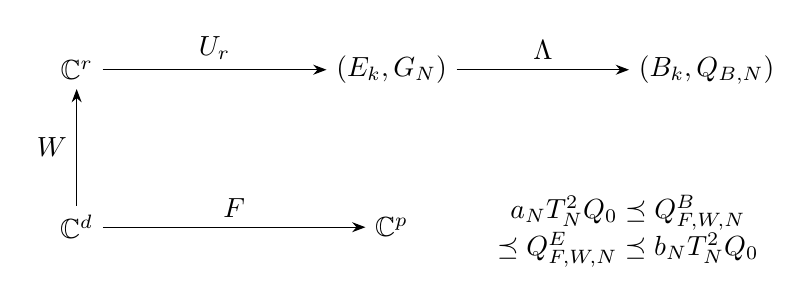
\begin{tikzpicture}[>=Stealth,scale=1]
\node (a) at (0,2) {$\mathbb C^r$};
\node (b) at (4,2) {$(E_k,G_N)$};
\node (c) at (8,2) {$(B_k,Q_{B,N})$};
\draw[->] (a)--node[above]{$U_r$}(b);
\draw[->] (b)--node[above]{$\Lambda$}(c);
\node (d) at (0,0) {$\mathbb C^d$};
\node (e) at (4,0) {$\mathbb C^p$};
\draw[->] (d)--node[left]{$W$}(a);
\draw[->] (d)--node[above]{$F$}(e);
\node[align=center] at (7,-.05)
 {$a_NT_N^2Q_0\preceq Q^B_{F,W,N}$\\
  $\preceq Q^E_{F,W,N}\preceq b_NT_N^2Q_0$};
\end{tikzpicture}
\caption{The original inverse-power frame and its literal observation
give the two metrics on $\mathbb C^r$. Restriction by $W$ followed by
the minimum over $F$ gives IFH4--7; the full metric $Q_0$ is retained.
The diagram introduces no replacement of the source or the conductor.
The diagram is exact, not a numerical sample.}
\end{figure}

\begin{thebibliography}{9}
\bibitem{IVO} Supplied continuation, \emph{The original observation
preserves an entire inverse-power determinant at the $kq$ scale},
equations (1)--(56), 21 September 2026. The complete mathematical text
and the independently derived finite IVO proof accompany this edition.
No human authorship is inferred from the supplied correspondence.
\bibitem{NG} Split-Zero research programme,
\emph{Gaussian spectral actions through the original arithmetic quotient},
\href{https://github.com/KokunoYumeto/zeta-function-research-reader/blob/5992ad50c0f2a06921f1fcaded7b4e38097c0739/workbenches/splitzero-tandem/continuations/20260920-original-kernel-mixed-determinants/providers/NATIVE_GAUSSIAN_TRANSFER.tex#L203}{NG10--16, complete original zero-law proof}.
\bibitem{Smallest} Supplied mathematical continuation,
\emph{The unique small singular direction of the native arithmetic quotient},
\href{https://github.com/KokunoYumeto/zeta-function-research-reader/blob/0fd693c844aad9117e30ec447c59864a28af10f3/workbenches/splitzero-tandem/continuations/20260921-native-spectral-real-pair/003/NATIVE_SMALLEST_SINGULAR_PROOF.tex}{S1--45, complete pinned proof and interval certificate}.
\bibitem{Profile} Supplied mathematical continuation,
\emph{Original-metric heat transitions and complete mixed-family control},
\href{https://github.com/KokunoYumeto/zeta-function-research-reader/blob/0fd693c844aad9117e30ec447c59864a28af10f3/workbenches/splitzero-tandem/continuations/20260921-native-spectral-real-pair/003/RETAINED_PROFILE_PROOF.tex}{H4--5, complete pinned source}.
\bibitem{LS} Split-Zero research programme,
\emph{The late heat direction through the original observation},
\href{https://github.com/KokunoYumeto/zeta-function-research-reader/blob/0fd693c844aad9117e30ec447c59864a28af10f3/workbenches/splitzero-tandem/continuations/20260921-native-spectral-real-pair/003/LATE_HEAT_ORIGINAL_KERNEL_RECEIVER.tex}{LS1--17, complete pinned proof}.
\bibitem{DLMF} T. H. Koornwinder, R. Wong, R. Koekoek,
R. F. Swarttouw, with W. P. Reinhardt, \emph{Orthogonal Polynomials},
NIST DLMF Chapter 18, version 1.2.8.
The original recurrence and generating function conventions are
\href{https://dlmf.nist.gov/18.22.E8}{18.22.E8} and
\href{https://dlmf.nist.gov/18.23.E7}{18.23.E7}.
The finite-kernel and parity steps are proved above and in the
accompanying finite derivation; no external asymptotic theorem replaces NG10.
\end{thebibliography}
\clearpage\part{Independent complete finite observation estimate}
\section{A finite original-metric comparison for the whole inverse-power frame}\label{a-finite-original-metric-comparison-for-the-whole-inverse-power-frame}

Independent derivation, 21 September 2026. Equations \textbf{IVO1--26} belong to this file. The received inverse-power observation manuscript, equations (14)--(38), is checked here from its finite source maps. Its finite estimates are valid on the stated domain. The arguments below fill its hard-gap, complex-kernel, nearby-degree and vector-uniform comparison steps. The selected-pole constant may be improved by taking the maximum over all actual nonzero conductor coefficients.

This proof does not use a monic-norm asymptotic, a limiting zero distribution, or the full root-value metric condition number. The original conductor coefficients and the entire observation kernel stay fixed.

\subsection{1. Original maps and the full minimum}\label{original-maps-and-the-full-minimum}

Fix \(0<\delta<1/2\), \(\gamma>2\), \(k\equiv1\bmod4\), and the original simple-quartet period domain. Put \[
q=(k+1)^2,\quad k_-=k-8,\quad q_-=(k-7)^2,\quad
\Delta=q-q_-=16k-48,\quad D_0=\sqrt{\delta^2+\gamma^2}.
\] The physical coordinate is \(S=k/2+iy\), and \[
Q_k(y)=\prod_{a,b=0}^k[y-(2b-k)\gamma+i(2a-k)\delta].
\] Its roots are distinct, nonzero, closed under negation and conjugation. Its real polynomial is even and has no real zeros. Keep the native source \(d\mu_k=w_h^{*k}(y)\,dy\) and the complete original observation \(\Lambda_k:E_k=\mathbb C[y]/(Q_k)\to B_k\), whose kernel \(K_k\) is the original invariant annihilator.

For each actual nonzero conductor coefficient \(a_j=a_{r_js_j}\), set \[
b_j=4+(2r_j-8)\delta+i(2s_j-8)\gamma,\qquad
\zeta_j=i(b_j-4),\quad J=\#\{j:a_j\ne0\},\quad A_1=\sum_j|a_j|.
\] The shifts are distinct, \(|\zeta_j|\le8D_0\), and \(|\zeta_i-\zeta_j|\ge2\delta\). The complete conductor symbol is \(E_A(z)=\sum_ja_je^{b_jz}\), with first nonzero moment \(\mu_v=E_A^{(v)}(0)\), \(v\le J-1\).

Writing \(\Psi_cf(S)=f((S-c)/i)\), \(c=k/2\), \(c'=c-4\), direct substitution gives \[
\Psi_{c'}^{-1}{\cal T}_A\Psi_cf(y)=\sum_ja_jf(y-\zeta_j).
\tag{IVO1}
\] Its symbol is \(e^{-4z/i}E_A(z/i)\), so its first nonzero derivative is \(i^{-v}\mu_v\); its leading coefficient on a monic degree-\(n\) polynomial is \(i^{-v}\mu_v\binom nv\). Every shifted lower root is an upper root. Thus IVO1 induces \(C_A:E_k\to E_-=\mathbb C[y]/(Q_-)\), with \(Q_-=Q_{k-8}\) in its own centered coordinate.

The original conductor theorem IK1--3 proves \(K_k\subseteq\ker C_A\). The exact induced map through the full observation is \[
\widehat C_A(\Lambda_k[p])=[{\cal T}_Ap]_{Q_-},\qquad
\widehat C_A\Lambda_k=C_A.
\tag{IVO2}
\] It is well defined precisely because of this inclusion; no equality of the two kernels is used.

Let \(G_N\) be the complete attained native metric for degrees \(\le N\), and let \(P_{B,N}=G_N^{-1}\Lambda_k^*Q_{B,N}\Lambda_k\), with \(Q_{B,N}=(\Lambda_kG_N^{-1}\Lambda_k^*)^{-1}\). By completing the positive quadratic form on each observed fibre, its norm is \[
\|P_{B,N}f\|_{G_N}
=\inf\{\|p\|_{\mu_k}:\deg p\le N,\ \Lambda_k[p]=\Lambda_kf\}.
\] Every such polynomial has the same conductor image \(C_Af\). NG2 supplies the original full-mass comparison \[
\ell_{k,N}\|p\|_\sigma^2\le\|p\|_{\mu_k}^2\le u_k\|p\|_\sigma^2,\qquad
\log(u_k/\ell_{k,N})=O_h(k+\log(N+1)).
\tag{IVO3}
\] Here \(d\sigma=|\Gamma(1/4+iy/2)|^2dy/(2\pi)\), with mass \(M_\sigma=\sqrt{2\pi}\). A quotient norm \(\|f\|_{\sigma,Q,L}\) means the minimum over polynomial representatives through degree \(L\). A rational expression specifies its quotient class only.

The Gamma generating function is \(\sum p_n(y)t^n/n!=(1+t^2)^{-1/4}e^{y\arctan t}\), with \(\gamma_n=M_\sigma n!(1/2)_n\). On \(|t|=N/(N+1)\), \[
|\Re\arctan t|\le\pi/4,\qquad
|\Im\arctan t|\le\tfrac12\log(2N+1).
\] These follow by writing \(\arctan t=(2i)^{-1}\log((1+it)/(1-it))\); the quotient has positive real part, and modulus between \((1-|t|)/(1+|t|)\) and its reciprocal. Translation by \(-\zeta_j\) multiplies the generating function by \(e^{-\zeta_j\arctan t}\). Cauchy's coefficient estimate through degree \(N\) costs at most \(e\), since \((1+1/N)^N\le e\). In the orthonormal basis its coefficient ratio is \(\rho_n/\rho_m\le\sqrt{2N+1}\), where \(\rho_n=\sqrt{n!/(1/2)_n}\), \(1\le\rho_n\le\sqrt{2n+1}\). Each triangular entry is therefore bounded by \(e^{1+2\pi\gamma}(2N+1)^{4\delta+1/2}\). Its norm is at most \((N+1)\) times that maximum, by the row and column sum inequality. Summing the actual coefficients proves \[
{\cal F}_N=A_1e^{1+2\pi\gamma}(N+1)(2N+1)^{4\delta+1/2},\quad
\|{\cal T}_A\|_{\mathcal P_N,\sigma}\le{\cal F}_N.
\] Taking the two original minima now gives \[
\|P_{B,N}f\|_{G_N}\ge
\frac{\sqrt{\ell_{k,N}}}{{\cal F}_N}\|C_Af\|_{\sigma,Q_-,N-v},
\qquad
\|f\|_{G_N}\le\sqrt{u_k}\|f\|_{\sigma,Q_k,N}.
\tag{IVO4}
\]

\subsection{2. Gamma multiplication and anchored division}\label{gamma-multiplication-and-anchored-division}

Set \(b_L=\sqrt{2L+1}\sum_{j=1}^L1/j\), \(b_0=0\). Differentiating the above generating function gives the exact orthonormal formula \[
\partial_y\phi_n=\sum_{\substack{1\le a\le n\\a\ {\rm odd}}}
\frac{(-1)^{(a-1)/2}}a\frac{\rho_n}{\rho_{n-a}}\phi_{n-a}.
\] Both its row and column sums through degree \(L\) are at most \(b_L\); hence \(\|\partial_y\|\le b_L\). Pairing \(\partial_y((y-z)p)-(y-z)\partial_yp=p\) with \(p\), moving multiplication to its actual adjoint \(y-\bar z\), and using equality of the two multiplication norms on the real line proves \[
\frac{\|p\|_\sigma}{2b_{L+1}}\le\|(y-z)p\|_\sigma
\le[2(L+1)+|z|]\|p\|_\sigma,\qquad \deg p\le L.
\tag{IVO5}
\] The upper bound uses the unchanged Gamma raising/lowering coefficients \(\sqrt{j(j-1/2)}\).

At zero, the generating function gives \[
M_\sigma|\phi_{2m}(0)|^2
=\frac{(1/2)_m(1/4)_m}{m!(3/4)_m}\le1,\qquad \phi_{2m+1}(0)=0.
\] Thus \(M_\sigma K_{\sigma,L}(0,0)\le L+1\). Applying IVO5 to \({\mathscr D}p=(p-p(0))/y\), which has degree \(\le L-1\), gives \[
\|{\mathscr D}p\|_\sigma
\le2b_L(1+\sqrt{L+1})\|p\|_\sigma=:\mathfrak d_L\|p\|_\sigma.
\tag{IVO6}
\] All powers of anchored division below act on polynomials; rational functions are never integrated.

\subsection{3. The hard gap, including its finite constants}\label{the-hard-gap-including-its-finite-constants}

The original-author Gamma product gives \[
\frac{\sigma(y)}{c_\sigma}
=\prod_{j=0}^\infty\left(1+\frac{(y/2)^2}{(j+1/4)^2}\right)^{-1},
\quad c_\sigma=\frac{\Gamma(1/4)^2}{2\pi}.
\] The factor at \(j=0\) is \(1+4y^2\). For \(a=|y|/2\), the decreasing positive function \(\log(1+a^2/x^2)\) satisfies \[
\sum_{j=1}^\infty\log(1+a^2/(j+1/4)^2)
\le\int_0^\infty\log(1+a^2/x^2)\,dx=\pi a.
\] The integral follows by integration by parts and \(\int_0^\infty (x^2+a^2)^{-1}dx=\pi/(2a)\), with its limiting value zero at \(a=0\). Therefore \[
\frac{c_\sigma e^{-\pi|y|/2}}{1+4y^2}\le\sigma(y)\le c_\sigma.
\tag{IVO7}
\]

Let \(Q\) be any monic degree-\(d\) polynomial, \(d\ge16\), whose roots have modulus at most \(c_*d\), \(c_*=2^{-13}\). For any polynomial \(p\) of degree \(\le2d\), compare the inner interval \(|y|\le c_*d\) with \([d,2d]\).

Here is the required Legendre estimate with no missing exponential constant. Rodrigues' polynomials on \([-1,1]\) satisfy \[
P_j(t)=2^{-j}\sum_{\ell=0}^j\binom j\ell^2(t-1)^{j-\ell}(t+1)^\ell,\qquad
\int_{-1}^1P_iP_j=\frac2{2j+1}\mathbf1_{i=j}.
\] The first identity is Leibniz's rule in \((2^jj!)^{-1}(d/dt)^j(t^2-1)^j\). Integration by parts \(j\) times proves orthogonality. Its leading coefficient is \((2j)!/(2^j(j!)^2)\); evaluating \(\int(1-t^2)^jdt=2^{2j+1}(j!)^2/(2j+1)!\) gives the displayed squared norm. For \(|y|\le c_*d\), \(t=2y/d-3\) has \(|t\pm1|<5\). The finite formula and \(\sum_\ell\binom j\ell^2=\binom{2j}j\le4^j\) give \(|P_j(t)|\le10^j\). Expanding \(p\) in the orthonormal basis \(\sqrt{(2j+1)/d}\,P_j(2y/d-3)\) of \([d,2d]\) proves \[
\sup_{|y|\le c_*d}|p(y)|^2
\le\frac{(2d+1)^2\,10^{4d}}d\int_d^{2d}|p(u)|^2\,du.
\tag{IVO8}
\]

On the inner interval \(|Q|\le(2c_*d)^d\); on \([d,2d]\), \(|Q|\ge(d/2)^d\). Using IVO7/8, the ratio of the inner \(Qp\)-mass to its mass on \([d,2d]\) is at most \[
2c_*(1+16d^2)(2d+1)^2
[16c_*^2\,10^4e^\pi]^d
<\frac{(1+16d^2)(2d+1)^2}{4096\,4^d}\le1.
\] The strict factor inequality follows from \(\pi<4,e<3\), since \(16\cdot2^{-26}\cdot10^4\cdot81<1/4\). The final sequence is decreasing for \(d\ge16\): its adjacent ratio is at most \(((d+1)/d)^4/4<1\), and its value at 16 is less than one. Since \([d,2d]\) is exterior to the inner interval, at least half the total mass is exterior. Hence \[
\int y^2|Qp|^2d\sigma\ge\beta_d\int|Qp|^2d\sigma,\qquad
\beta_d=2^{-27}d^2,\qquad\deg p\le2d.
\tag{IVO9}
\]

\subsection{4. Exact consequences for complex evaluation kernels}\label{exact-consequences-for-complex-evaluation-kernels}

Suppose \(|Q|^2d\sigma\) is even, and let \(\lambda\) be its full pushforward under \(x=y^2\). Denote the monic orthogonal polynomials for \(d\lambda\) and \(x\,d\lambda\) by \(P_j^0,P_j^1\). The even orthogonal polynomials in \(y\) are \(P_j^0(y^2)\); the odd ones are \(yP_j^1(y^2)\), with exactly their original norms.

IVO9 gives a Rayleigh lower bound \(\beta_d\) for multiplication by \(x\) on the finite polynomial spaces for each of these two measures. For the first, use \(p(y)=f(y^2)\); for the second, use \(p(y)=yf(y^2)\). Zeros of a monic degree-\(j\) orthogonal polynomial are the eigenvalues of the compressed multiplication by \(x\) on degrees below \(j\): expansion in an orthonormal basis gives the tridiagonal recurrence, whose determinant recurrence is the monic polynomial recurrence. Thus all zeros in \(x\) that occur for \(y\)-degree \(\le2d-1\) are at least \(\beta_d\). This proves the zero bound from the gap, rather than presuming zero location from parity.

For \(|z|\le R\), paired-zero factorization gives \[
|\phi_{2j}^{(Q)}(z)|^2
\le e^{2jR^2/\beta_d}|\phi_{2j}^{(Q)}(0)|^2.
\] For the odd sum, factor \(P_j^1(z^2)\) in the same way. The form inequality \(\int x|f|^2d\lambda\ge\beta_d\int|f|^2d\lambda\) implies, by inversion of its finite positive Gram, that the \(x\,d\lambda\) evaluation kernel at zero is at most \(\beta_d^{-1}\) times the \(d\lambda\) kernel of the same degree. Summing even and odd terms, with all parity cutoffs retained, therefore proves \[
K_{Q,n}(z,z)\le e^{nR^2/\beta_d}
(1+R^2/\beta_d)K_{Q,n}(0,0),\qquad n\le2d-2.
\tag{IVO10}
\] This inequality holds at complex \(z\), not only on the real line.

For even \(n\le2d-2\), let \(H_{Q,n}(y)=K_{Q,n}(y,0)/K_{Q,n}(0,0)\). It has value one at zero and squared weighted norm \(K_{Q,n}(0,0)^{-1}\). Reproduction shows \(yH_{Q,n}\) is orthogonal to degrees \(\le n-1\); parity supplies degree \(n\) as well. Its leading coefficient is nonzero, since the highest even orthogonal polynomial has nonzero value at zero. Thus it is a nonzero scalar multiple of the monic odd polynomial of degree \(n+1\). Its nonzero squared zeros are at least \(\beta_d\). If \(R^2\le\beta_d/2\), paired factorization and \(\log(1-u)\ge-2u\) for \(0\le u\le1/2\) give \[
|H_{Q,n}(z)|\ge e^{-nR^2/\beta_d},\qquad |z|\le R.
\tag{IVO11}
\]

\subsection{5. Nearby relation degrees}\label{nearby-relation-degrees}

Assume every root of \(Q\) has imaginary part of modulus at least \(\delta\). For \(\deg p\le n+1\), \[
\|p'\|_{|Q|^2\sigma}
\le\|(Qp)'\|_\sigma+\|(Q'/Q)Qp\|_\sigma
\le V\|p\|_{|Q|^2\sigma},\quad
V=b_{d+n+1}+d/\delta.
\] For the derivative application at degrees through \(n\), this displayed \(V\) is more than sufficient. Multiplication through those degrees has norm at most \(U=2(d+n+2)\), by applying the original Gamma multiplication bound to \(Qp\). If \(a_j\) denotes the orthonormal recurrence coefficient, the coefficient of \(\phi_{j-1}\) in \(\phi_j'\) is \(j/a_j\); hence \(a_j\ge j/V\), and multiplication gives \(a_j\le U\). Evenness makes the diagonal recurrence coefficient zero, so \(\phi_{j+2}(0)=-(a_{j+1}/a_{j+2})\phi_j(0)\). For even \(n_0\le n\), only even degrees contribute at zero, proving \[
\begin{gathered}
K_{Q,n}(0,0)\le{\cal D}_{d;n_0,n}K_{Q,n_0}(0,0),\\
{\cal D}_{d;n_0,n}=
\prod_{t=1}^{\lfloor n/2\rfloor-n_0/2}
\left[1+\left(\frac{UV}{n_0+2t}\right)^2\right].
\end{gathered}\tag{IVO12}
\] Each step bounds the new squared value by \((UV/(n_0+2t))^2\) times the preceding squared value, which is at most the preceding kernel. No orthogonality or source metric is changed.

\subsection{6. A polynomial representative of every inverse-power vector}\label{a-polynomial-representative-of-every-inverse-power-vector}

Take \(1\le r\le q\), \(d=(d_1,\ldots,d_r)\), and \(U_rd=\sum_{j=1}^rd_j[y^{-j}]\). Set \[
n_0=2\left\lfloor\frac{N+1-q}{2}\right\rfloor,\quad
T_N=\frac1{|Q_k(0)|\sqrt{K_{Q_k,n_0}(0,0)}},\quad
A_d(y)=\sum_{j=1}^rd_jy^{r-j},\quad H=H_{Q_k,n_0}.
\] Let \[
h(y)=-H(y)\operatorname{rem}_{y^r}\frac{A_d(y)}{Q_k(y)H(y)},\qquad
p(y)=\frac{A_d(y)+Q_k(y)h(y)}{y^r}.
\tag{IVO13}
\] The denominator has nonzero constant term, so its Taylor truncation is well defined. The numerator vanishes to order at least \(r\), and \(\deg p\le q+n_0-1\le N\). Modulo \(Q_k\), it equals \(U_rd\). Moreover its first \(r\) coefficients in \(Q_kh\) are exactly \(-A_d\), so \(p={\mathscr D}^r(Q_kh)\). This is an exact polynomial source lift.

Put \(\rho=\delta/2<1\) and \[
{\cal Q}_\rho=\prod_{\omega/\pm}
(1-\rho^2/|\omega|^2)^{-1}.
\] Negation pairs give \(|Q_k(0)/Q_k(z)|\le{\cal Q}_\rho\) on \(|z|=\rho\). To bound it, let the positive odd coordinate indices be \(i,j\le k\). Then \[
\sum_{\omega/\pm}\frac1{|\omega|^2}
\le\frac2{\delta^2}\sum_{\substack{i,j\le k\\i,j\ {\rm odd}>0}}\frac1{i^2+j^2}
\le\frac2{\delta^2}\sum_{\substack{j\le k\\j\ {\rm odd}>0}}\frac1j.
\] The last inequality groups terms by \(\max(i,j)=j\); there are \(j\) terms on that shell, each at most \(j^{-2}\). Since \(\rho^2/|\omega|^2\le1/4\), \(-\log(1-u)\le2u\) proves \[
\log{\cal Q}_\rho\le
\frac{4\rho^2}{\delta^2}\sum_{\substack{j\le k\\j\ {\rm odd}>0}}\frac1j.
\tag{IVO14}
\] On \(|z|=\rho\), \(|A_d(z)|\le\|d\|_2/\sqrt{1-\rho^2}\). IVO11 and Cauchy's estimate bound the \(j\)-th truncated Taylor coefficient in IVO13 by \[
\frac{{\cal Q}_\rho e^{n_0\rho^2/\beta_q}}
{|Q_k(0)|\sqrt{1-\rho^2}}\,\rho^{-j}\|d\|_2.
\] Multiply the actual polynomial \(Q_kH\) by \(y^j\), applying IVO5 at every intermediate degree, and then apply IVO6 \(r\) times. All degrees are at most \(N+r\). This proves \[
\begin{gathered}
\|U_rd\|_{\sigma,Q_k,N}\le{\cal U}_{r,N}T_N\|d\|_2,\\
{\cal U}_{r,N}=
\mathfrak d_{N+r}^{\,r}
\frac{{\cal Q}_\rho e^{n_0\rho^2/\beta_q}}{\sqrt{1-\rho^2}}
\sum_{j=0}^{r-1}\left(\frac{2(N+r+1)}{\rho}\right)^j.
\end{gathered}\tag{IVO15}
\]

\subsection{7. The complete conductor pole and all coefficient directions}\label{the-complete-conductor-pole-and-all-coefficient-directions}

The rational quotient response in the physical lower coordinate is \[
C_AU_rd=[R_d]_{Q_-},\quad
R_d(y)=\sum_{j=1}^J\sum_{n=1}^r\frac{a_jd_n}{(y-\zeta_j)^n}.
\tag{IVO16}
\] This follows from IVO1 at every lower root and retains the original physical \(i\) through that coordinate map. No pole \(\zeta_j\) is a lower root, because its imaginary coordinate is an even multiple of \(\delta\), whereas every lower root has an odd multiple.

Put \(B(y)=\prod_j(y-\zeta_j)^r\), \(A_d^-=BR_d\). Any degree-\((N-v)\) polynomial representative \(p\) of this class satisfies \[
Bp-A_d^-=Q_-h,\qquad
\deg h\le n_-:=N-v+Jr-q_-.
\tag{IVO17}
\] At an actual pole \(\zeta_*\), let \(B_*=\prod_{j\ne*}(y-\zeta_j)^r\). The degree-\(<r\) Taylor jet at \(\zeta_*\) of \(Q_-h/B_*\) equals \[
-a_*(d_r,d_{r-1},\ldots,d_1).
\tag{IVO18}
\] Indeed \(Bp/B_*=(y-\zeta_*)^rp\), and all other terms of \(A_d^-/B_*\) vanish to order \(r\) at this pole. This exact triangular identity prevents cancellation of any inverse-power coefficient by other poles.

Let \(m_0=r(J-1)\) and define \(t_j^{(m_0)}=\binom{m_0+j-1}{j}(2\delta)^{-m_0-j}\) for \(m_0>0\), while \(t_0^{(0)}=1\), \(t_j^{(0)}=0\) for \(j>0\). Every normalized derivative coefficient of \(Q_-\) at \(\zeta_*\) is bounded by \(|Q_-(\zeta_*)|\binom{q_-}{\ell}\delta^{-\ell}\), by the product formula and the separation from lower roots. The coefficients of \(1/B_*\) are bounded by \(t_j^{(m_0)}\), by multiplying the binomial series of all its factors. Hence the jet multiplication operator has two-norm at most \(|Q_-(\zeta_*)|{\cal P}\), where \[
{\cal P}=\sum_{j=0}^{r-1}\sum_{\ell=0}^j
\binom{q_-}{\ell}\delta^{-\ell}t_{j-\ell}^{(m_0)}.
\] This follows since a truncated Toeplitz convolution has operator norm at most its coefficient one-norm, by extending by zero and the triangle inequality.

Use IVO10 on \(|z-\zeta_*|=\rho\) and Cauchy's formula. The coefficient-jet norm of \(h\) is at most \[
{\cal E}_*\sqrt{K_{Q_-,n_-}(0,0)}\|Q_-h\|_\sigma,\quad
{\cal E}_*=\sqrt r\,\rho^{1-r}
e^{n_-(|\zeta_*|+\rho)^2/(2\beta_{q_-})}
\sqrt{1+(|\zeta_*|+\rho)^2/\beta_{q_-}}.
\] Here \(\rho<1\) bounds all the coefficient factors \(\rho^{-j}\) by \(\rho^{1-r}\). Define \({\cal L}_*=|a_*|/({\cal P}{\cal E}_*)\). IVO18 now proves \[
\|Q_-h\|_\sigma\ge
\frac{{\cal L}_*\|d\|_2}
{|Q_-(\zeta_*)|\sqrt{K_{Q_-,n_-}(0,0)}}.
\tag{IVO19}
\]

All numerator terms also remain. With \(Z=\max_j|\zeta_j|\), put \[
{\cal B}=2(N-v+Jr+1)+Z,\qquad
{\cal A}=\sqrt{M_\sigma}A_1\sqrt r[2(Jr+1)+Z]^{Jr-1}.
\] Each term of \(A_d^-\) is a product of \(Jr-n\le Jr-1\) retained linear factors. Repeated IVO5, starting from the constant polynomial of norm \(\sqrt{M_\sigma}\), and \(\sum_n|d_n|\le\sqrt r\|d\|_2\), show \[
\|A_d^-\|_\sigma\le{\cal A}\|d\|_2,\qquad
\|Bp\|_\sigma\le{\cal B}^{Jr}\|p\|_\sigma.
\tag{IVO20}
\]

\subsection{8. Compare the original relation kernels before estimating their size}\label{compare-the-original-relation-kernels-before-estimating-their-size}

The centered lower grid is exactly the central subset of the upper grid: \(Q_k=Q_-D_\partial\), \(\deg D_\partial=\Delta\). Set \({\cal W}=2(q+n_0+1)+kD_0\). Repeated IVO5 on all \(\Delta\) boundary factors gives \(\|Q_kp\|_\sigma\le{\cal W}^{\Delta}\|Q_-p\|_\sigma\) for degree \(\le n_0\). Inverting the two finite positive Grams yields \(K_{Q_-,n_0}(0,0)\le{\cal W}^{2\Delta}K_{Q_k,n_0}(0,0)\). Apply IVO12 to the first kernel. With \[
{\cal R}_*=
\frac{|Q_k(0)|}
{|Q_-(\zeta_*)|{\cal W}^{\Delta}
\sqrt{{\cal D}_{q_-;n_0,n_-}}},
\] one obtains the exact comparison \[
\frac1{|Q_-(\zeta_*)|\sqrt{K_{Q_-,n_-}(0,0)}}
\ge{\cal R}_*T_N.
\tag{IVO21}
\] The nearby-degree hypotheses hold: \(n_-\ge n_0\), since \(v\le J-1\) and \(\Delta>0\).

Every boundary root has at least one odd coordinate of modulus \(\ge k-6\), so \(|D_\partial(0)|\ge[\delta(k-6)]^\Delta\). Negation pairing and the shell sum used in IVO14 give \[
\left|\frac{Q_-(\zeta_*)}{Q_-(0)}\right|
\le\exp\left[\frac{2|\zeta_*|^2}{\delta^2}
\sum_{\substack{j\le k-8\\j\ {\rm odd}>0}}\frac1j\right].
\] There are \(O(k+Jr)\) nearby-degree factors in IVO12, each with logarithm \(O_A(\log(q+Jr+2))\). Therefore \[
\log^+(1/{\cal R}_*)=O_A((k+Jr)\log(q+Jr+2)).
\tag{IVO22}
\] This argument explicitly retains the boundary product rather than assigning a loss by rank alone.

\subsection{9. Finite absorption guard and the uniform frame sandwich}\label{finite-absorption-guard-and-the-uniform-frame-sandwich}

The elementary Legendre estimate IVO8, now on \([q,2q]\) and evaluated at zero for degree \(n_0\), gives \[
|H(0)|^2\le\frac{(n_0+1)^2\,10^{2n_0}}q\int_q^{2q}|H(y)|^2dy.
\] Since \(H(0)=1\), all \(Q_k\)-roots have modulus \(\le R_k=kD_0\), and IVO7 holds, the exact relation norm satisfies \[
T_N\ge T_N^{\rm lb}:=
\frac{\sqrt{c_\sigma q/(1+16q^2)}(q-R_k)^q e^{-\pi q/2}}
{|Q_k(0)|(n_0+1)10^{n_0}}.
\tag{IVO23}
\]

Use the finite domain \[
q_-\ge16,\quad R_k\le2^{-14}q_-,\quad
n_-+2\le2q_-,\quad
{\cal L}_*{\cal R}_*T_N^{\rm lb}\ge2{\cal A}.
\tag{IVO24}
\] It puts both relation polynomials in IVO9's root radius, all kernels in IVO10--12's degree range, and \(\rho^2\le\beta_q/2\). In fact \(|\zeta_*|+\rho\le R_k\) here, so the complex-disc ratios are bounded by \(1/2\) as well. The upper source \(n_0\le q\) also meets its degree range.

From IVO17, \(\|Q_-h\|\le\|Bp\|+\|A_d^-\|\). Combining IVO19--24 absorbs the entire numerator error and proves, for every representative \(p\), \[
\|p\|_\sigma\ge
\frac{{\cal L}_*{\cal R}_*}{2{\cal B}^{Jr}}T_N\|d\|_2.
\] Take its actual quotient minimum, then apply IVO4 and IVO15. The resulting finite positive factor is \[
\boxed{
\frac{\|P_{B,N}U_rd\|_{G_N}^2}{\|U_rd\|_{G_N}^2}
\ge\vartheta_{r,N,*}:=
\frac{\ell_{k,N}}{u_k}
\left[\frac{{\cal L}_*{\cal R}_*}
{2{\cal F}_N{\cal B}^{Jr}{\cal U}_{r,N}}\right]^2
}\qquad(d\ne0).
\tag{IVO25}
\] Every quantity is finite and specified. Any actual pole satisfying its own absorption guard may be used. Taking the maximum of these \(\vartheta_{r,N,*}\) gives a valid stronger finite factor \(\vartheta_{r,N}\); a vanishing conductor coefficient is never substituted by a nonzero one.

For \(r\log(q+2)=o(q)\), fixed original \(A,h,\delta,\gamma\), each displayed logarithmic cost is \(O_{h,A}((k+Jr)\log(q+Jr+2))\). Indeed the binomial jet factors have indices \(<r\), the degree-change product has \(O(k+Jr)\) terms, and the multiplication/anchored-division factors have polynomial bases and \(O(Jr+r)\) exponents. The complex-kernel exponent is \(O_A(n_-/q_-^2)=O_A(1/q)\). On the other hand IVO23 and \(|Q_k(0)|\le R_k^q\) imply \(\log T_N^{\rm lb}\ge q\log(q/k)-O_h(q)\). Thus the absorption guard eventually holds, uniformly in \(q-1\le N\le2q\). The other finite guards hold eventually as well.

The original inverse-power frame is independent for \(r\le q\): multiply a purported zero combination by \(y^r\), use invertibility of \(y\) modulo \(Q_k\), and note that \(A_d\) has degree \(<r\le q\). Its full Gram \(H^E_{r,N}\) is therefore positive. IVO25 gives positivity of its observed Gram \(H^B_{r,N}\) without a rank inference. Since the observation minimum is a contraction, the vector-uniform conclusion is \[
\boxed{\begin{gathered}
e^{-C_{h,A}(k+Jr)\log(q+Jr+2)}H^E_{r,N}
\preceq H^B_{r,N}\preceq H^E_{r,N},\\
0\le\log\frac{\det H^E_{r,N}}{\det H^B_{r,N}}
\le C_{h,A}r(k+Jr)\log(q+Jr+2).\end{gathered}
}\tag{IVO26}
\] For the determinant inequality apply the positive congruence by \((H^E)^{-1/2}\) and multiply its \(r\) eigenvalue bounds. That final factor \(r\) is justified only after proving the same finite estimate on every original coefficient vector.

The same derivation gives an absolute sandwich around the common factor \(T_N^2\|d\|^2\): its upper side is \(u_k{\cal U}_{r,N}^2T_N^2\|d\|^2\); its observed lower side is \(\ell_{k,N}({\cal L}_*{\cal R}_*/(2{\cal F}_N{\cal B}^{Jr}))^2T_N^2\|d\|^2\). This is the exact finite input needed for the receiving four-cutoff determinant calculation. No limiting coefficient has been used to prove it.

\subsection{Exact auxiliary verification}\label{exact-auxiliary-verification}

The accompanying check\_inverse\_power\_observation.py passes \textbf{45 exact checks}, recorded in INVERSE\_POWER\_OBSERVATION\_CHECKS.json. They verify the hard-gap scalar allowances; finite positive gap minors for an even degree-16 relation satisfying the root-radius condition; the anchored value and odd orthogonality of three exact reproducing minimum polynomials; physical shifts on the actual \(k=9\) upper/lower grids; both retained pole jets for a two-coefficient conductor; and an exact degree-\(99\) lift of an inverse-power vector modulo the complete degree-\(100\) original \(Q_9\). The \(k=9\) checks assert the finite algebra only; this small grid does not satisfy the eventual hard-gap guard. No computed native determinant or asymptotic is claimed by these fixtures.

\subsection{Sources, exact versions, and proof scope}\label{sources-exact-versions-and-proof-scope}

\begin{itemize}
\tightlist
\item
  \textbf{R. A. Askey and R. Roy}, DLMF Chapter 5, version 1.2.8 released 2026-09-15, \href{https://dlmf.nist.gov/5.8.E3}{Gamma product 5.8.E3}, \href{https://dlmf.nist.gov/5.8.E3.tex}{original TeX}. Complete original equation read and retained in graph\_primary\_sources/DLMF\_5\_8\_E3\_Gamma\_product\_original.tex. The explicit envelope IVO7 is derived here from it.
\item
  \textbf{T. H. Koornwinder, R. Wong, R. Koekoek, R. F. Swarttouw, with W. P. Reinhardt}, DLMF Chapter 18, \href{https://dlmf.nist.gov/18.23.E7}{Meixner--Pollaczek generating function 18.23.E7}, \href{https://dlmf.nist.gov/18.22.E8}{recurrence 18.22.E8}, and \href{https://dlmf.nist.gov/18.12.E11}{Legendre generating function 18.12.E11}. The last equation's original TeX was retained and read; IVO8 proves its needed finite Legendre estimate explicitly. IVO10--12 prove the parity and kernel consequences directly. Source reading scope and hashes are in graph\_primary\_sources/IVO\_PRIMARY\_READING\_RECEIPT.json.
\item
  Programme \textbf{Complete conductor graph metric}, CG7--11, \href{https://github.com/KokunoYumeto/zeta-function-research-reader/blob/0fd693c844aad9117e30ec447c59864a28af10f3/workbenches/splitzero-tandem/continuations/20260921-native-spectral-real-pair/003/COMPLETE_CONDUCTOR_GRAPH_METRIC.tex}{complete pinned public proof}. Its exact Gamma polynomial convention is used in IVO4--6.
\item
  Programme \textbf{Gaussian spectral actions through the original arithmetic quotient}, NG1--3, \href{https://github.com/KokunoYumeto/zeta-function-research-reader/blob/5992ad50c0f2a06921f1fcaded7b4e38097c0739/workbenches/splitzero-tandem/continuations/20260920-original-kernel-mixed-determinants/providers/NATIVE_GAUSSIAN_TRANSFER.tex\#L32}{complete pinned public proof}. Its source comparison NG2, including original full-mass constants, was read for IVO3.
\item
  Programme \textbf{The original conductor detects a full inverse-power space}, IK1--12, \href{https://github.com/KokunoYumeto/zeta-function-research-reader/blob/689a8f87e9c12b7a99b01b3123438c6751ee608f/workbenches/splitzero-tandem/continuations/20260921-directional-inverse-power/007/INVERSE_POWER_CONDUCTOR_OBSERVABILITY.tex}{complete pinned IK proof}, supplies the actual invariant-kernel inclusion. Its physical shifts and induced quotient map are reproduced in IVO1--2, and its pole mechanism in IVO16--19. The full source also accompanies this edition.
\item
  The supplied inverse-power observation manuscript, equations (1)--(56), was read completely from the retained supplied mathematical source. This independent proof verifies the finite estimates (14)--(38) and their original-map receivers (8)--(13). Its asymptotic coefficient, heat consequences and eigenclass conclusions are proved separately in IFH1--21 of this edition, with their complete inherited source proofs.
\end{itemize}

\clearpage\part{The complete supplied continuation}
\subsection{\texorpdfstring{The original observation preserves an entire inverse-power determinant at the \(kq\) scale}{The original observation preserves an entire inverse-power determinant at the kq scale}}\label{the-original-observation-preserves-an-entire-inverse-power-determinant-at-the-kq-scale}

Retain the simple-quartet domain

\[
0<\delta<\frac12,\qquad \gamma>2,\qquad k\equiv1\pmod4,
\qquad q=(k+1)^2,
\]

the complete polynomial

\[
Q_k(y)=
\prod_{a,b=0}^{k}
\bigl[y-(2b-k)\gamma+i(2a-k)\delta\bigr],
\]

and multiplication \(M_k[P]=[yP]\) on \(E_k=\mathbb C[y]/(Q_k)\).

At each original cutoff \(q-1\le N\le2q\), let \(G_N\) be the attained metric of the original source \(w_h^{*k}\). Let

\[
\Lambda_k:E_k\longrightarrow B_k,\qquad
Q_{B,N}=(\Lambda_kG_N^{-1}\Lambda_k^*)^{-1},
\]

be the unchanged observation and its full minimum metric, and put

\[
P_{B,N}=G_N^{-1}\Lambda_k^*Q_{B,N}\Lambda_k.
\]

For \(1\le r\le q\), define the literal inverse-power frame

\[
U_r d=\sum_{j=1}^{r}d_j[y^{-j}],
\]

and its two Grams

\[
H^E_{r,N}=U_r^*G_NU_r,\qquad
H^B_{r,N}=U_r^*\Lambda_k^*Q_{B,N}\Lambda_kU_r.
\tag{1}
\]

These are the powers of the original \(M_k^{-1}\), subsequently observed. They are not inverse powers of an independently compressed observed operator.

The current conductor theorem proves finite injectivity on these spaces, but its displayed metric lower bound can involve the full root-value metric condition number. The following calculation replaces that factor on the specified inverse-power space. The exact conductor and kernel inclusion used here are IK1--IK12 at the inspected commit \nolinkurl{fe22dc1dd51c633e82f93b731cbb6ec96b11ed64}.

\textbf{Theorem.} Fix the original period and its nonzero conductor coefficients. Let \(J\) be their number. Suppose

\[
r=r(k)\ge1,\qquad r\log(q+2)=o(q).
\]

Then, uniformly over the original cutoff window,

\[
\boxed{
e^{-C_{h,A}(k+Jr)\log(q+Jr+2)}H^E_{r,N}
\preceq H^B_{r,N}\preceq H^E_{r,N}.
}
\tag{2}
\]

In particular,

\[
\boxed{
0\le
\log\det H^E_{r,N}-\log\det H^B_{r,N}
\le
C_{h,A}\,r(k+Jr)\log(q+Jr+2).
}
\tag{3}
\]

A finite, explicitly specified lower factor replacing the exponential in (2) is derived below. The finite estimate uses the original polynomial-norm comparison, but \textbf{does not use the monic-profile asymptotic or the equilibrium zero law}.

For the evaluated determinant limit, retain those two additional inputs, exactly as in the supplied smallest-singular-value proof. Then, with

\[
\mathcal R F_N=F_{q-1}+F_q-F_{2q-1}-F_{2q},
\]

one obtains

\[
\boxed{
\lim_{k\to\infty}\frac{1}{rq}\mathcal R\log\det H^B_{r,N}
=
\lim_{k\to\infty}\frac{1}{rq}\mathcal R\log\det H^E_{r,N}
=
\mathfrak C,
}
\tag{4}
\]

where

\[
\boxed{
\mathfrak C
=
4\left[\psi(0)-\psi(1)-J(1)-1\right].
}
\tag{5}
\]

Here \(\psi\) and \(J\) retain the definitions in the preceding proof:

\[
\psi(0)=\log(4/\pi),\qquad
J(s)=(1+s)[\log(1+s)-1]
-\frac{s}{2}\int\log x\,\rho_s(x)\,dx.
\]

The supplied interval certificate therefore gives

\[
\boxed{
\frac{1353893}{10^6}<\mathfrak C<
\frac{1354751}{10^6}.
}
\tag{6}
\]

This enclosure is inherited from that certificate, not a new numerical run.

Taking \(r=k\) in particular evaluates the requested growing-rank scale:

\[
\boxed{
\mathcal R\log\det
\bigl(U_k^*\Lambda_k^*Q_{B,N}\Lambda_kU_k\bigr)
=
\mathfrak C\,kq+o_h(kq).
}
\tag{7}
\]

The full original kernel has not been replaced. Its additional constraints enter through the actual \(P_{B,N}\); the estimate below holds for every vector in this fixed inverse-power space.

\begin{center}\rule{0.5\linewidth}{0.5pt}\end{center}

\subsection{1. The conductor comparison is between the actual value maps}\label{the-conductor-comparison-is-between-the-actual-value-maps}

Write

\[
k_-=k-8,\qquad q_-=(k-7)^2,\qquad
\Delta=q-q_-=16k-48,
\]

and let \(Q_-=Q_{k-8}\), in its own centred \(y\)-coordinate.

For the nonzero original coefficients \(a_j\), retain

\[
b_j=4+(2r_j-8)\delta+i(2s_j-8)\gamma,
\qquad
\zeta_j=i(b_j-4).
\]

Thus

\[
|\zeta_j|\le8\sqrt{\delta^2+\gamma^2},
\qquad
|\zeta_i-\zeta_j|\ge2\delta\quad(i\ne j).
\]

The two physical centres are

\[
c=k/2,\qquad c'=c-4.
\]

For \(\Psi_cf(S)=f((S-c)/i)\), direct substitution gives

\[
\boxed{
\Psi_{c'}^{-1}\mathcal T_A\Psi_cf(y)
=
\sum_j a_jf(y-\zeta_j).
}
\tag{8}
\]

In particular, the \(i^n\) in the original \(S\)-coordinate inverse powers cancels through the displayed coordinate map, not by deleting a phase.

Let \(v=\operatorname{ord}_0E_A\). The centred symbol is

\[
e^{-4z/i}E_A(z/i),
\]

so its first nonzero derivative is \(i^{-v}\mu_v\). The operator in (8) lowers degree by exactly \(v\), with leading coefficient

\[
i^{-v}\mu_v\binom nv
\]

on a monic degree-\(n\) polynomial.

Denote its induced quotient map by \(C_A\). The exact source identities are

\[
J_-\mathcal T_A=C_AJ_N,
\qquad
K_k:=\ker\Lambda_k\subseteq\ker C_A.
\tag{9}
\]

Equivalently, there is a well-defined map

\[
\widehat C_A:B_k\longrightarrow \mathbb C[y]/(Q_-),
\qquad
\widehat C_A(\Lambda_k[p])=[\mathcal T_Ap]_{Q_-}.
\]

These are the original conductor identities; no equality between the full observation kernel and the conductor kernel is assumed.

For any quotient class \(f\), write

\[
\|f\|_{\sigma,Q,L}
=
\min_{\substack{p\in\mathcal P_L\\p=f\pmod Q}}\|p\|_\sigma.
\]

When \(f\) is rational with denominator coprime to \(Q\), this denotes its polynomial quotient class. \textbf{No rational function is integrated across its poles.}

The original native comparison is

\[
\ell_{k,N}\|p\|_\sigma^2
\le\|p\|_{\mu_k}^2
\le u_k\|p\|_\sigma^2,
\qquad
\log(u_k/\ell_{k,N})=O_h(k+\log(N+1)).
\tag{10}
\]

Its full-mass constants are the retained NG2 constants.

A useful explicit forward bound for (8) is

\[
\boxed{
\|\mathcal T_A\|_{\sigma,\mathcal P_N\to\mathcal P_{N-v}}
\le
\mathcal F_N
:=
A_1e^{1+2\pi\gamma}(N+1)(2N+1)^{4\delta+1/2},
\qquad A_1=\sum_j|a_j|.
}
\tag{11}
\]

It follows from the unchanged Gamma generating function

\[
\sum_{n\ge0}\frac{p_n(y)}{n!}t^n
=(1+t^2)^{-1/4}e^{y\arctan t}.
\]

Translation multiplies it by \(e^{-\zeta_j\arctan t}\). On \(|t|=N/(N+1)\),

\[
|\Re\arctan t|<\pi/4,\qquad
|\Im\arctan t|\le\tfrac12\log(2N+1).
\]

Cauchy's coefficient bound costs at most \(e\), and the original orthonormal coefficient ratio is at most \(\sqrt{2N+1}\). Summing the \(N+1\) diagonals and all \(a_j\) proves (11). The generating-function convention is DLMF 18.23.7. (\href{https://dlmf.nist.gov/18.23}{DLMF})

Now minimize over the \textbf{same original observed fibre}. Every admissible native representative \(p\) has

\[
C_A[p]=C_Af.
\]

Consequently,

\[
\boxed{
\|P_{B,N}f\|_{G_N}
\ge
\frac{\sqrt{\ell_{k,N}}}{\mathcal F_N}
\|C_Af\|_{\sigma,Q_-,N-v},
}
\tag{12}
\]

whereas

\[
\boxed{
\|f\|_{G_N}
\le\sqrt{u_k}\|f\|_{\sigma,Q_k,N}.
}
\tag{13}
\]

The rest of the proof compares the two polynomial minima in (12)--(13) \textbf{before estimating their common exponentially large factor}.

\subsection{2. Finite control of the reference relation kernels}\label{finite-control-of-the-reference-relation-kernels}

For a polynomial \(Q\), let

\[
\mathsf K_{Q,n}(z,w)
=
\sum_{j=0}^{n}\phi_j^{(Q)}(z)
\overline{\phi_j^{(Q)}(w)}
\]

be the reproducing kernel for degree at most \(n\) in

\[
|Q(y)|^2d\sigma(y).
\]

The measure is not divided by its mass.

Set

\[
b_L=\sqrt{2L+1}\sum_{j=1}^{L}\frac1j,\qquad b_0=0.
\]

The Gamma derivative formula gives

\[
\|\partial_y\|_{\mathcal P_L,\sigma}\le b_L.
\]

Pairing

\[
[\partial_y,y-z]p=p
\]

with \(p\), and retaining the adjoint multiplication by \(y-\bar z\), yields

\[
\boxed{
\frac{\|p\|_\sigma}{2b_{L+1}}
\le\|(y-z)p\|_\sigma
\le[2(L+1)+|z|]\|p\|_\sigma.
}
\tag{14}
\]

These are the full-polynomial bounds CG9--CG11 in the current source.

For anchored division

\[
\mathscr Dp=\frac{p-p(0)}y,
\]

the original evaluation kernel at zero gives

\[
\boxed{
\|\mathscr D\|_{\mathcal P_L,\sigma}
\le
\mathfrak d_L:=2b_L(1+\sqrt{L+1}).
}
\tag{15}
\]

\subsubsection{A hard gap allowing twice the relation degree}\label{a-hard-gap-allowing-twice-the-relation-degree}

Let \(Q\) be monic of degree \(d\ge16\), with all roots in

\[
|z|\le2^{-13}d.
\]

Then, for every polynomial \(p\) of degree at most \(2d\),

\[
\boxed{
\int y^2|Qp|^2\,d\sigma
\ge\beta_d\int|Qp|^2\,d\sigma,
\qquad
\beta_d=2^{-27}d^2.
}
\tag{16}
\]

Here is a finite proof. Put \(c_*=2^{-13}\) and

\[
c_\sigma=\frac{\Gamma(1/4)^2}{2\pi}.
\]

Euler's product gives

\[
\frac{c_\sigma e^{-\pi|y|/2}}{1+4y^2}
\le\sigma(y)\le c_\sigma.
\tag{17}
\]

The product and its convention are those of DLMF §5.8. (\href{https://dlmf.nist.gov/5.8}{DLMF})

On \(|y|\le c_*d\),

\[
|Q(y)|\le(2c_*d)^d;
\]

on \([d,2d]\),

\[
|Q(y)|\ge(d/2)^d.
\]

The Legendre evaluation estimate on \([1,2]\) gives, for \(\deg p\le2d\),

\[
\sup_{|y|\le c_*d}|p(y)|^2
\le
\frac{(2d+1)^2\,10^{4d}}{d}
\int_d^{2d}|p(u)|^2\,du.
\]

Therefore the ratio of the inner mass to the mass on \([d,2d]\) is at most

\[
2c_*(1+16d^2)(2d+1)^2
\left(16c_*^2\,10^4e^\pi\right)^d.
\]

Using \(\pi<4\) and \(e<3\), the factor in parentheses is below \(1/4\). Thus the ratio is bounded by

\[
\frac{(1+16d^2)(2d+1)^2}{4096\,4^d}\le1.
\]

At least half the full mass lies outside \(|y|\le c_*d\), proving (16).

\subsubsection{Kernel consequences}\label{kernel-consequences}

Assume now that \(|Q|^2d\sigma\) is even. Within the degree range just established,

\[
\boxed{
\mathsf K_{Q,n}(z,z)
\le
e^{nR^2/\beta_d}
\left(1+\frac{R^2}{\beta_d}\right)
\mathsf K_{Q,n}(0,0),
\qquad |z|\le R.
}
\tag{18}
\]

Indeed every nonzero squared zero of the relevant even or odd orthogonal polynomial is at least \(\beta_d\). For even degrees, factor the polynomial into its paired zeros and use \(1+x\le e^x\). For odd degrees, write the polynomial as \(y\) times an orthogonal polynomial for the \(x\)-weighted pushforward measure. Equation (16) compares that whole weighted Gram with \(\beta_d\) times the unweighted one. Summing the even and odd evaluations gives (18). The reproducing-kernel and parity identities used here have the standard conventions of DLMF §18.2. (\href{https://dlmf.nist.gov/18.2}{DLMF})

For even \(n\), define the exact minimum polynomial

\[
H_{Q,n}(y)=
\frac{\mathsf K_{Q,n}(y,0)}{\mathsf K_{Q,n}(0,0)}.
\]

It satisfies

\[
H_{Q,n}(0)=1,\qquad
\|QH_{Q,n}\|_\sigma^2=\mathsf K_{Q,n}(0,0)^{-1},
\]

and, when \(R^2\le\beta_d/2\),

\[
\boxed{
|H_{Q,n}(z)|\ge e^{-nR^2/\beta_d},
\qquad |z|\le R.
}
\tag{19}
\]

To see the zero structure exactly, \(yH_{Q,n}\) is a scalar multiple of the original odd monic polynomial of degree \(n+1\). Its nonzero zeros obey (16).

One also needs to compare nearby kernel degrees. If all roots of \(Q\) have imaginary part of modulus at least \(\delta\), then

\[
\|p'\|_{|Q|^2\sigma}
\le
\left(b_{d+n+1}+\frac d\delta\right)
\|p\|_{|Q|^2\sigma}.
\]

The first term differentiates \(Qp\); the second uses

\[
|Q'(y)/Q(y)|\le d/\delta
\]

on the real line.

Put

\[
V=b_{d+n+1}+d/\delta,\qquad U=2(d+n+2).
\]

The monic recurrence coefficients obey \(a_j\ge j/V\) and \(a_j\le U\). Therefore, for even \(n_0\le n\), with \(h=\lfloor n/2\rfloor-n_0/2\),

\[
\boxed{
\mathsf K_{Q,n}(0,0)
\le
\mathcal D_{d;n_0,n}\,\mathsf K_{Q,n_0}(0,0),
}
\tag{20}
\]

where the entirely finite factor is

\[
\boxed{
\mathcal D_{d;n_0,n}
=
\prod_{t=1}^{h}
\left[
1+\left(\frac{UV}{n_0+2t}\right)^2
\right].
}
\tag{21}
\]

This follows from the exact even evaluation recurrence

\[
\phi_{j+2}(0)
=-\frac{a_{j+1}}{a_{j+2}}\phi_j(0).
\]

\subsection{3. A uniform norm comparison for every inverse-power coefficient vector}\label{a-uniform-norm-comparison-for-every-inverse-power-coefficient-vector}

Put

\[
n_0=2\left\lfloor\frac{N+1-q}{2}\right\rfloor,
\qquad
T_N=
\frac1{|Q_k(0)|\sqrt{\mathsf K_{Q_k,n_0}(0,0)}}.
\tag{22}
\]

This is the common large factor.

\subsubsection{The source upper bound}\label{the-source-upper-bound}

Let

\[
A_d(y)=\sum_{j=1}^{r}d_jy^{r-j},
\qquad
H=H_{Q_k,n_0}.
\]

In the formal Taylor ring at zero, define

\[
h(y)=
-H(y)\operatorname{rem}_{y^r}
\frac{A_d(y)}{Q_k(y)H(y)}.
\]

Then

\[
p(y)=\frac{A_d(y)+Q_k(y)h(y)}{y^r}
\]

is a polynomial of degree at most \(N\), and

\[
[p]_{Q_k}=U_rd.
\]

This is a representative in the original polynomial source.

Take \(\rho=\delta/2\), and choose one root from each pair \(\{\omega,-\omega\}\) of \(Q_k\). Define

\[
\mathcal Q_\rho
=
\prod_{\omega/\pm}
\left(1-\frac{\rho^2}{|\omega|^2}\right)^{-1}.
\]

On \(|y|=\rho\),

\[
|Q_k(0)/Q_k(y)|\le\mathcal Q_\rho.
\]

Moreover,

\[
\log\mathcal Q_\rho
\le
\frac{4\rho^2}{\delta^2}
\sum_{\substack{1\le j\le k\\j\ {\rm odd}}}\frac1j
=O(\log k).
\tag{23}
\]

Cauchy's coefficient estimate, (19), repeated multiplication by \(y\), and (15) now give

\[
\boxed{
\|U_rd\|_{\sigma,Q_k,N}
\le \mathcal U_{r,N}T_N\|d\|_2,
}
\tag{24}
\]

with

\[
\boxed{
\mathcal U_{r,N}
=
\mathfrak d_{N+r}^{\,r}
\frac{\mathcal Q_\rho e^{n_0\rho^2/\beta_q}}
{\sqrt{1-\rho^2}}
\sum_{j=0}^{r-1}
\left(\frac{2(N+r+1)}{\rho}\right)^j.
}
\tag{25}
\]

The cancellation at zero is exact:

\[
p=\mathscr D^r(Q_kh).
\]

Thus (24) never integrates \(y^{-r}\).

\subsubsection{The conductor lower bound retains every pole}\label{the-conductor-lower-bound-retains-every-pole}

In the centred lower coordinate,

\[
C_AU_rd
=
\left[
R_d(y)
\right]_{Q_-},
\qquad
R_d(y)=
\sum_{j=1}^{J}\sum_{n=1}^{r}
\frac{a_jd_n}{(y-\zeta_j)^n}.
\tag{26}
\]

Put

\[
B(y)=\prod_{j=1}^{J}(y-\zeta_j)^r,
\qquad
A_d^-(y)=B(y)R_d(y).
\]

If \(p\) is any degree-\((N-v)\) representative of this lower quotient class, then

\[
Bp-A_d^-=Q_-h,
\qquad
\deg h\le n_-:=N-v+Jr-q_-.
\tag{27}
\]

Fix one actual nonzero coefficient \(a_*\), at its actual pole \(\zeta_*\), and let

\[
B_*(y)=\prod_{j\ne *}(y-\zeta_j)^r.
\]

The full divided jet of (27) at that pole is

\[
\boxed{
\operatorname{jet}_{\zeta_*,<r}
\left(\frac{Q_-h}{B_*}\right)
=
-a_*\,(d_r,d_{r-1},\ldots,d_1).
}
\tag{28}
\]

All other rational summands are analytic at \(\zeta_*\) and become divisible by \((y-\zeta_*)^r\). This is why their interference cannot erase the coefficient vector in (28).

Here are finite constants for the resulting estimate. For \(m_0=r(J-1)\), define

\[
t_j^{(m_0)}=
\begin{cases}
\displaystyle
\binom{m_0+j-1}{j}(2\delta)^{-m_0-j},&m_0>0,\\
1,&m_0=0,\ j=0,\\
0,&m_0=0,\ j>0,
\end{cases}
\]

and

\[
\mathcal P
=
\sum_{j=0}^{r-1}\sum_{\ell=0}^{j}
\binom{q_-}{\ell}\delta^{-\ell}
t_{j-\ell}^{(m_0)}.
\tag{29}
\]

This bounds the full triangular multiplication on the jet in (28), after retaining \(|Q_-(\zeta_*)|\).

Equation (18) and Cauchy's formula give

\[
\mathcal E
=
\sqrt r\,\rho^{1-r}
e^{n_-(|\zeta_*|+\rho)^2/(2\beta_{q_-})}
\sqrt{1+\frac{(|\zeta_*|+\rho)^2}{\beta_{q_-}}},
\qquad
\mathcal L=\frac{|a_*|}{\mathcal P\mathcal E}.
\tag{30}
\]

Therefore

\[
\|Q_-h\|_\sigma
\ge
\frac{\mathcal L\|d\|_2}
{|Q_-(\zeta_*)|
 \sqrt{\mathsf K_{Q_-,n_-}(0,0)}}.
\tag{31}
\]

Let \(Z=\max_j|\zeta_j|\), and put

\[
\mathcal B=2(N-v+Jr+1)+Z,
\]

\[
\mathcal A
=
\sqrt{\mathfrak m_\sigma}\,A_1\sqrt r
[2(Jr+1)+Z]^{Jr-1},
\qquad \mathfrak m_\sigma=\sqrt{2\pi}.
\]

The complete numerator satisfies

\[
\|A_d^-\|_\sigma\le\mathcal A\|d\|_2,
\qquad
\|Bp\|_\sigma\le\mathcal B^{Jr}\|p\|_\sigma.
\]

Thus (27)--(31) give a lower bound on the complete polynomial minimum, not on one selected representative.

\subsubsection{Compare the two relation kernels before bounding their size}\label{compare-the-two-relation-kernels-before-bounding-their-size}

The central lower grid is an exact subset of the upper grid:

\[
Q_k=Q_-D_{\partial},\qquad \deg D_\partial=\Delta.
\]

Set

\[
\mathcal W=2(q+n_0+1)+k\sqrt{\delta^2+\gamma^2},
\]

and

\[
\boxed{
\mathcal R_*=
\frac{|Q_k(0)|}
{|Q_-(\zeta_*)|\,
 \mathcal W^\Delta
 \sqrt{\mathcal D_{q_-;n_0,n_-}}}.
}
\tag{32}
\]

Repeated application of the full multiplication bound (14), followed by (20), proves

\[
\frac1{|Q_-(\zeta_*)|
\sqrt{\mathsf K_{Q_-,n_-}(0,0)}}
\ge \mathcal R_*T_N.
\tag{33}
\]

Every removed root remains in (32). For the size estimate, the removed grid consists of the four outer odd shells, so

\[
|D_\partial(0)|\ge[\delta(k-6)]^\Delta.
\]

Also, pairing the lower roots gives

\[
\left|\frac{Q_-(\zeta_*)}{Q_-(0)}\right|
\le
\exp\left[
\frac{2|\zeta_*|^2}{\delta^2}
\sum_{\substack{1\le j\le k-8\\j\ {\rm odd}}}\frac1j
\right].
\]

Together with (21),

\[
\log^+(1/\mathcal R_*)
=
O_A((k+Jr)\log(q+Jr+2)).
\tag{34}
\]

The large factor \(T_N\) has a fully explicit lower bound. Put

\[
R_k=k\sqrt{\delta^2+\gamma^2}.
\]

Evaluation on \([q,2q]\), with all Gamma and polynomial factors retained, yields

\[
\boxed{
T_N\ge T_N^{\rm lb}:=
\frac{
\sqrt{c_\sigma q/(1+16q^2)}\,
(q-R_k)^q e^{-\pi q/2}
}{
|Q_k(0)|(n_0+1)10^{n_0}
}.
}
\tag{35}
\]

A sufficient finite domain is

\[
q_-\ge16,\qquad
R_k\le2^{-14}q_-,
\qquad
n_-+2\le2q_-,
\]

together with

\[
\boxed{\mathcal L\mathcal R_*T_N^{\rm lb}\ge2\mathcal A.}
\tag{36}
\]

All quantities in these guards are specified above or are the original conductor coefficients.

On that domain, (27)--(36) prove

\[
\boxed{
\|C_AU_rd\|_{\sigma,Q_-,N-v}
\ge
\frac{\mathcal L\mathcal R_*}
{2\mathcal B^{Jr}}T_N\|d\|_2.
}
\tag{37}
\]

Combining (12), (13), (24), and (37) gives the promised finite observation factor:

\[
\boxed{
\frac{\|P_{B,N}U_rd\|_{G_N}^2}
{\|U_rd\|_{G_N}^2}
\ge
\frac{\ell_{k,N}}{u_k}
\left[
\frac{\mathcal L\mathcal R_*}
{2\mathcal F_N\mathcal B^{Jr}\mathcal U_{r,N}}
\right]^2.
}
\tag{38}
\]

For \(r\log(q+2)=o(q)\), every logarithmic factor on the right costs

\[
O_{h,A}((k+Jr)\log(q+Jr+2)).
\]

Meanwhile

\[
\log T_N^{\rm lb}
\ge q\log(q/k)-O_h(q).
\]

Consequently the finite guard (36) eventually holds, and (38) proves (2)--(3).

The pole argument itself permits repeated roots. For another packet, however, the full-jet conductor factorization, nested polynomial comparison, and actual kernel inclusion must be retained for that packet; they are not inferred from its reduced root set.

\subsection{4. Evaluation of the determinant coefficient}\label{evaluation-of-the-determinant-coefficient}

The preceding bounds give, for both \(H^E_{r,N}\) and \(H^B_{r,N}\),

\[
\log\det H_{r,N}
=
r\log u_k
-2r\log|Q_k(0)|
-r\log\mathsf K_{Q_k,n_0}(0,0)
+
O_{h,A}\!\left(r(k+Jr)\log(q+Jr+2)\right).
\tag{39}
\]

At the four original cutoffs, \(n_0\) is exactly

\[
0,\ 0,\ q,\ q.
\]

The common source factor \(u_k\) and the full root product \(Q_k(0)\) therefore cancel under the prescribed signs:

\[
\boxed{
\mathcal R\log\det H_{r,N}
=
2r\log
\frac{\mathsf K_{Q_k,q}(0,0)}
     {\mathsf K_{Q_k,0}(0,0)}
+o_{h,A}(rq).
}
\tag{40}
\]

It remains to evaluate one reference-kernel ratio.

Let \(U_n^\Gamma\) be the monic polynomials for \(Q_k^2d\sigma\), with squared norms \(\nu_n^\Gamma\). Christoffel--Darboux at zero gives

\[
\mathsf K_{Q_k,q}(0,0)
=
\frac{U_{q+1}^{\Gamma\,\prime}(0)U_q^\Gamma(0)}
{\nu_q^\Gamma}.
\]

The ratio

\[
\Xi_q=
\frac{U_{q+1}^{\Gamma\,\prime}(0)}{U_q^\Gamma(0)}
\]

satisfies

\[
1\le\Xi_q\le
\frac{4(2q+1)^2}{\beta_q}.
\tag{41}
\]

Indeed, after \(x=y^2\), the numerator and denominator are the values at zero of monic polynomials for \(x\,d\lambda\) and \(d\lambda\). Their zeros interlace in the positive interval supplied by (16). The product of their zero ratios is bounded by the largest zero divided by the smallest. Thus \(\log\Xi_q=O(1)\).

Since

\[
\mathsf K_{Q_k,0}(0,0)=1/\nu_0^\Gamma,
\]

we have the exact identity

\[
\boxed{
\log\frac{\mathsf K_{Q_k,q}(0,0)}
{\mathsf K_{Q_k,0}(0,0)}
=
2\log|U_q^\Gamma(0)|
+\log\nu_0^\Gamma-\log\nu_q^\Gamma+\log\Xi_q.
}
\tag{42}
\]

The original native/Gamma comparison passes to both complete monic affine minima. Hence the supplied H4 profile implies the same ratio estimate in the Gamma reference:

\[
\log\frac{\nu_j^\Gamma}{\omega_{q+j}^\Gamma}
=
2q\psi(j/q)+O_h(k\log^2(q+2)).
\tag{43}
\]

This is the precise use of the imported monic-profile input.

The full reference zero law, now applicable to the logarithm because of (16), gives

\[
\log|U_q^\Gamma(0)|
=
q\log q+\frac q2\int\log x\,\rho_1(x)\,dx+o_h(q).
\]

This is the same reference logarithmic limit used in the supplied proof.

Finally,

\[
\omega_n^\Gamma=\sqrt{2\pi}\,n!(1/2)_n
\]

gives

\[
\log\omega_{2q}^\Gamma-\log\omega_q^\Gamma
=
2q\log q+4q\log2-2q+O(\log q).
\]

Substitute into (42):

\[
\boxed{
\frac1q\log
\frac{\mathsf K_{Q_k,q}(0,0)}
{\mathsf K_{Q_k,0}(0,0)}
\longrightarrow
2[\psi(0)-\psi(1)-J(1)-1].
}
\tag{44}
\]

Equations (40) and (44) prove (4)--(7).

The estimate is on every vector in the inverse-power frame. The determinant conclusion is not inferred from a full-space volume comparison.

\subsection{5. The actual observed late-heat return has an eventual positive sign}\label{the-actual-observed-late-heat-return-has-an-eventual-positive-sign}

The current source identifies the late-heat line as

\[
u=-Q_k(0)[y^{-1}],
\]

and proves

\[
M_k^{-1}=B_N-\frac{u\varphi_N}{Q_k(0)},
\qquad
\|B_N\|\le D_N,
\qquad
E_N=\frac{\|u\|\|\varphi_N\|}{|Q_k(0)|}.
\]

If \(E_N>2D_N\), its smallest-singular projection \(P_{\min,N}\) satisfies

\[
\|P_{\min,N}-P_{u,N}\|_1
\le2\eta_N,\qquad
\eta_N=\frac{D_N}{E_N-D_N}.
\]

This is the inherited LS1--LS5 line estimate.

Our \(r=1\) bound gives the actual observed fraction

\[
\theta_N=
\frac{\|P_{B,N}u\|_{G_N}^2}{\|u\|_{G_N}^2}
\]

the new quantitative lower bound

\[
\boxed{
e^{-C_{h,A}k\log(q+2)}
\le\theta_N\le1.
}
\tag{45}
\]

In particular,

\[
\boxed{\frac1q\log\theta_N\longrightarrow0.}
\tag{46}
\]

This does not assert that \(\theta_N\) tends to a nonzero constant.

Define the measured full heat

\[
\Theta_N(\tau)
=
\operatorname{Tr}_{B_k}
\left[
\Lambda_k e^{-\tau M_k^{\dagger_{G_N}}M_k}
L_{B,N}
\right],
\qquad
L_{B,N}=G_N^{-1}\Lambda_k^*Q_{B,N}.
\tag{47}
\]

Equivalently,

\[
\Theta_N(\tau)
=
\operatorname{Tr}_{E_k}
\left[P_{B,N}e^{-\tau M_k^\dagger M_k}\right].
\]

This is the original observation of the full heat operator. It is not the heat trace of \(\Lambda_kM_kL_{B,N}\).

Let \(s_{\min,N}\) be the actual smallest singular value. The finite relative error is

\[
\boxed{
\left|
\frac{\Theta_N(\tau)}
{\theta_N e^{-\tau s_{\min,N}^2}}-1
\right|
\le
\frac{2\eta_N}{\theta_N}
+
\frac{q-1}{\theta_N}
e^{-\tau(D_N^{-2}-s_{\min,N}^2)}.
}
\tag{48}
\]

At the late times

\[
\tau_k(b)=\exp\{2q[\log(q/k)+b]\},
\]

both terms tend to zero. The reason is quantitative: the supplied smallest-singular theorem gives

\[
\eta_N=\exp[-q\log(q/k)+O_h(q)],
\]

whereas (45) loses only \(\exp[-O_{h,A}(k\log q)]\). Therefore

\[
\boxed{
\Theta_N(\tau_k(b))
=
\theta_N e^{-\tau_k(b)s_{\min,N}^2}(1+o_h(1)).
}
\tag{49}
\]

The observed line is also determined in relative trace norm. If

\[
\Pi_{\Lambda u,N}
=
\frac{(\Lambda u)(\Lambda u)^*Q_{B,N}}
{(\Lambda u)^*Q_{B,N}(\Lambda u)},
\]

then the measured heat, divided by its own trace, approaches this actual projector. No limiting observation angle is inserted.

For the same physical time used in the supplied four-cutoff theorem,

\[
\boxed{
\tau_k^*
=
\exp\left\{
2q\left[
\log(q/k)-1-\frac{I(\delta,\gamma)}2
\right]
\right\},
}
\tag{50}
\]

the lower two full heat weights tend to one, while the upper two are doubly exponentially small. The source's endpoint inequalities are

\[
\psi(1)+J(1)<-1<\psi(0)+J(0).
\]

They are retained without modification.

Since the observed lower weights are bounded below by (45),

\[
\boxed{
\mathcal R\Theta_N(\tau_k^*)>0
\quad\text{for all sufficiently large }k,
}
\tag{51}
\]

and more precisely

\[
\boxed{
\frac1q\log\bigl(\mathcal R\Theta_N(\tau_k^*)\bigr)
\longrightarrow0.
}
\tag{52}
\]

The limit of the unscaled signed trace is not assigned the value \(2\): its retained fractions \(\theta_N\) may still decay. What is established is its eventual sign and its complete leading exponential rate.

\subsection{6. The same logarithmic rate holds for every conductor-detected eigenclass}\label{the-same-logarithmic-rate-holds-for-every-conductor-detected-eigenclass}

There is a second application that does not require summing over projections.

For an upper root \(\lambda\), let

\[
e_\lambda(y)=
\frac{Q_k(y)}{(y-\lambda)Q_k'(\lambda)}
\]

be the actual cardinal eigenclass. Put

\[
\mathcal J_\lambda=
\{j:\mu_j:=\lambda+\zeta_j
\text{ is a lower root}\}.
\]

Then

\[
C_Ae_\lambda(\mu_j)=a_j,
\]

and the other lower values vanish. Thus

\[
C_Ae_\lambda\ne0
\iff\mathcal J_\lambda\ne\varnothing.
\tag{53}
\]

The different \(j\)'s give different lower roots, so these values do not cancel.

Define

\[
B_\lambda(y)=\prod_{j\in\mathcal J_\lambda}(y-\mu_j),
\qquad
Q_\lambda=\frac{Q_k}{y-\lambda},
\qquad
Q_{\mathrm{rest}}=\frac{Q_-}{B_\lambda},
\]

\[
n_a=N+1-q,\qquad
n_\lambda=N-v-q_-+|\mathcal J_\lambda|.
\]

The complete source minimum is

\[
\|e_\lambda\|_{\sigma,Q_k,N}^2
=
\frac1{|Q_k'(\lambda)|^2
\mathsf K_{Q_\lambda,n_a}(\lambda,\lambda)}.
\]

At any chosen \(j_*\in\mathcal J_\lambda\), the conductor image satisfies the finite lower bound obtained by retaining its exact value at \(\mu=\mu_{j_*}\). Therefore

\[
\boxed{
\begin{aligned}
\frac{\|P_{B,N}e_\lambda\|_{G_N}^2}
{\|e_\lambda\|_{G_N}^2}
\ge{}&
\frac{\ell_{k,N}}{u_k\mathcal F_N^2}\\
&\times
\frac{
|a_{j_*}|^2|B_\lambda'(\mu)|^2
|Q_k'(\lambda)|^2
\mathsf K_{Q_\lambda,n_a}(\lambda,\lambda)
}{
|Q_-'(\mu)|^2
\mathsf K_{Q_{\mathrm{rest}},n_\lambda}(\mu,\mu)
}.
\end{aligned}
}
\tag{54}
\]

Every kernel in (54) is a finite Gamma-polynomial kernel with its specified full factor. No native midpoint Gram is used.

To estimate the ratio, use

\[
Q_k(y)=Q_-(y+\zeta_{j_*})D_{j_*}(y),
\qquad
\frac{|Q_k'(\lambda)|}{|Q_-'(\mu)|}
=|D_{j_*}(\lambda)|
\ge(2\delta)^\Delta,
\]

and

\[
|B_\lambda'(\mu)|\ge(2\delta)^{|\mathcal J_\lambda|-1}.
\]

Multiplication bounds compare \(Q_\lambda\) and \(Q_{\mathrm{rest}}\) with the complete even polynomials; (18)--(21) compare their evaluation kernels. Since \(|\lambda|,|\mu|\le R_k=O_h(k)\) and \(\beta_q\asymp q^2\), the complex-point kernel factors cost only bounded or polynomial factors. This proves

\[
\boxed{
\frac{\|P_{B,N}e_\lambda\|_{G_N}^2}
{\|e_\lambda\|_{G_N}^2}
\ge e^{-C_{h,A}k\log(q+2)}
}
\tag{55}
\]

uniformly over all \(\lambda\) satisfying (53).

For any one nonzero conductor coefficient, its translated lower grid already contains \(q_-\) upper roots. Thus (55) applies to at least \(q_-\) of the \(q\) original eigenlines. It is an individual-line statement; it does not assert the same bound for arbitrary combinations of all those eigenvectors.

Finally, the cofactor minimum and the same kernel estimates give

\[
\log\|e_\lambda\|_{G_N}^2
=
\log u_k-2\log|Q_k'(\lambda)|
-\log\mathsf K_{Q_k,n_0}(0,0)
+O_h(k+\log q),
\]

uniformly over the full upper grid. The derivative factor is independent of \(N\). Consequently every conductor-detected eigenclass has the evaluated observed return

\[
\boxed{
\frac1q\mathcal R
\log\|P_{B,N}e_\lambda\|_{G_N}^2
\longrightarrow\mathfrak C.
}
\tag{56}
\]

Any original nonzero physical scalar attached to that eigenline cancels under the same four signs. For a terminal corner, the sufficient conductor condition is its actual corresponding corner coefficient being nonzero; a zero coefficient is not replaced by a generic one.

\begin{center}\rule{0.5\linewidth}{0.5pt}\end{center}

The matrices evaluated here are the original observed inverse-power Grams (1) and the original observed eigenclass norms. Their \(kq\)- and \(q\)-scale coefficients are now explicit. They are not reidentifications of the different invariant-kernel matrix \(I_K^*G_NI_K\), nor of the independently minimized proper-source target.

The finite estimates are the displayed polynomial, kernel, and pole inequalities. The limiting coefficient and late-time consequences additionally use the named source profile and reference zero law. No new numerical native-moment evaluation or machine-check execution is asserted.

\subsubsection{References}\label{references}

National Institute of Standards and Technology. (n.d.). \emph{Digital Library of Mathematical Functions}. §§5.8, 18.2, and 18.23. The Gamma product, reproducing-kernel conventions, parity transformation, and Meixner--Pollaczek generating function are used as identified above. (\href{https://dlmf.nist.gov/5.8}{DLMF})

\emph{Original-metric heat transitions and complete mixed-family control}. (2026, September 20). {[}User-supplied research manuscript{]}. H4--H5 supply the retained monic-norm profile and its stated scope.

Split-Zero research programme. (2026a, September 21). \emph{The original conductor detects a full inverse-power space} {[}Research manuscript, IK1--IK12; SZ-20260921-007{]}. \emph{Zeta-function research reader}, inspected at commit \nolinkurl{fe22dc1dd51c633e82f93b731cbb6ec96b11ed64}.

Split-Zero research programme. (2026b, September 21). \emph{Original conductor roots, native singular directions, and complete observation receivers} {[}Research manuscript, CG9--CG11 and LS1--LS7{]}. Same repository and inspected commit.

\emph{The unique small singular direction of the native arithmetic quotient}. (2026, September 21). {[}Supplied predecessor proof, S1--S45{]}. Its endpoint integral enclosure and late-time theorem are retained as separately identified inputs.

\end{document}
